\documentclass[11pt,a4paper]{article}

% ----- core typesetting -----
\usepackage[utf8]{inputenc}
\usepackage[T1]{fontenc}
\usepackage{lmodern}
\usepackage{microtype}
\usepackage[english]{babel}

% ----- math -----
\usepackage{amsmath}
\usepackage{amssymb}
\usepackage{amsthm}
\usepackage{mathtools}

% ----- figures and tables -----
\usepackage{graphicx}
\usepackage{booktabs}
\usepackage{array}
\usepackage{xcolor}
\usepackage{float}
\usepackage{enumitem}
\usepackage{tikz}
\usetikzlibrary{positioning,arrows.meta,fit,backgrounds,shapes.geometric}

% ----- authorship / layout -----
\usepackage{authblk}
\usepackage[margin=1in]{geometry}
\usepackage{setspace}

% ----- refs and hyperlinks (hyperref last among layout pkgs) -----
\usepackage[colorlinks=true,
            linkcolor=blue!60!black,
            citecolor=blue!60!black,
            urlcolor=blue!60!black,
            pdftitle={Syniscopy: A Shared-Scene Fisher-Information Framework for Comparing Single-Particle Imaging Systems},
            pdfauthor={Michael A. Khanna},
            pdfsubject={Synthetic single-particle microscopy simulator and Fisher information diagnostics},
            pdfkeywords={single-particle microscopy, Fisher information, Cramer-Rao lower bound, microscopy simulation, synthetic data}]{hyperref}
\usepackage{xurl}
\usepackage{cleveref}

% ----- bibliography -----

\newcommand{\generatedfallbackfigure}[3]{%
  \PackageError{syniscopy}{Required figure asset missing: #1}{Missing required figure file.}%
}

\newcommand{\generatedfallbacktable}[3]{%
  \PackageError{syniscopy}{Required table asset missing: #1}{Missing required table file.}%
}

% Convenience shortcut for contribution callouts used in the intro.
\newcommand{\contrib}[1]{\textbf{(#1)}}
\newtheorem{theorem}{Theorem}
\newtheorem{corollary}{Corollary}
\newtheorem{proposition}{Proposition}
\theoremstyle{remark}
\newtheorem{remark}{Remark}

% -------------------------------------------------------------------------
% Title block
% -------------------------------------------------------------------------
\title{Syniscopy: A Shared-Scene Fisher-Information Framework\\
       for Comparing Single-Particle Imaging Systems}

\author{Michael A. Khanna\thanks{Correspondence:
  \href{mailto:michael.a.khanna@vanderbilt.edu}{michael.a.khanna@vanderbilt.edu}.
  ORCID: \href{https://orcid.org/0009-0000-1458-0729}{0009-0000-1458-0729}.}}

\date{May 25, 2026}

% Formatting helper for long prose / path-like tokens
\setlength{\emergencystretch}{2em}

\begin{document}
\maketitle

\begin{abstract}
\begin{abstract}
Syniscopy is a shared-scene Fisher-information diagnostic for comparing configured nanoparticle microscopes under explicit forward-model assumptions. The unit of comparison is a \emph{microscope}: a chosen contrast modality, which fixes the physics backend, together with that instrument's own complete optical, detector, and backend configuration. Two microscopes may select the same modality yet differ entirely in their parameters, and instrument quantities such as numerical aperture or pupil sampling belong to a microscope rather than to a modality. The method maps multiple configured microscopes onto a common rigid-particle scene parameterization, including lateral position, axial position, and local \(\mathrm{SE}(3)\) pose coordinates, then computes Cramer--Rao diagnostics per microscope: lateral derivatives use the exact spectral gradient of the sampled band-limited contrast image, while axial and orientation derivatives remain explicit symmetric rerenders. The workflow emits status-gated artifacts for microscope ranking, detected-quanta normalization, algebraic fusion, and supervision-mask policy checks. Comparing bare modalities is recovered as the special case of fixing one instrument and varying only its contrast modality. The central claim is not a universal benchmark ordering; it is that comparisons are interpretable only after the scene, instrument configuration, measurement domain, noise model, and derivative contract are fixed. We demonstrate the workflow on configured optical and electron profile cards, native-regime source-provenance audits, and deterministic supervision-policy cases. Headline paper artifacts are tied to explicit sampling, convergence, and validation-status files so lateral undersampling/support failures and axial/orientation derivative gates remain visible rather than being hidden in prose.
\end{abstract}

\end{abstract}

\section{Introduction}

A nanoparticle image is not an intrinsic measurement of ``modality quality''. It is the result of a scene, a configured instrument, a forward model, detector units, noise assumptions, and a derivative convention. Syniscopy makes those choices explicit by putting multiple configured microscopes on one shared scene parameterization and then emitting the Fisher-information diagnostics, status flags, and provenance needed to interpret comparisons under that parameterization.

We define a \emph{microscope} as the unit that the Cram\'{e}r--Rao bound is computed on: a chosen contrast modality together with that instrument's own complete parameter set. The modality selects the physics backend and contrast mechanism (for example a fluorescence emission backend, or an electron-transport backend); the instrument-level parameters --- numerical aperture, pixel pitch, pupil sampling, wavelength, detector noise, dose, and backend-specific settings --- belong to the microscope, not to the modality. Consequently two microscopes can select the same modality and still differ entirely in their configurations, and a parameter that is meaningless for one modality is simply absent from microscopes that do not use it. Comparing modalities directly is then a derived special case: hold one instrument fixed and vary only the contrast modality, with each variant evaluated using only the parameters its modality consumes.

The contribution is not a new microscope forward model for every modality. It is a shared-scene information contract: one latent particle/sample state is rendered through multiple declared microscope configurations, differentiated on the same physical parameter frame, and reported with sampling, convergence, validation, fusion, normalization, and supervision metadata. The paper-facing outputs are lateral and axial Cramer--Rao diagnostics, \(\mathrm{SE}(3)\) rank and symmetry checks, detected-quanta-normalized comparisons, algebraic fusion and serial-allocation diagnostics, and supervision masks whose positive/ignore labels are gated by measurement support. Lateral localization uses a step-free spectral derivative; axial and orientation diagnostics keep the explicit rerendered perturbation checks required by those state axes.

We use the term \emph{contract} for an evaluation view: Contract-LP fixes lateral particle-position diagnostics, Contract-LZ fixes axial diagnostics, Contract-Q fixes detected-quanta normalization, and Contract-NR fixes native-regime source-use auditing. A contract is not a benchmark leaderboard. It states what is being optimized and which artifacts must pass before a row can be treated as validated.

The manuscript is therefore organized around the minimum load-bearing evidence: the shared-scene formulation, the symmetry/fusion consequences, the matched-microscope-packet implementation, the supervision policy, and demonstrations whose generated artifacts expose sampling, convergence, and provenance status.

\section{Related Work}
\label{sec:related}

Existing simulators address important parts of this problem: multi-modality rendering, fluorescence-cell simulation, bacterial-cell synthetic training data, point-emitter benchmarks, and high-fidelity interference-microscopy simulation. DeepTrack and DeepTrack~2 \cite{deeptrack} provide a compositional framework for bright-field, dark-field, interferometric-scattering, holography, and fluorescence simulations, with Mie scatterers and flexible sample/optics pipelines. CytoPacq \cite{cytopacq} targets fluorescence-cell imaging with acquisition-artifact modeling, and SyMBac \cite{symbac} uses synthetic micrographs to train bacterial-cell segmentation models. Single-molecule localization microscopy benchmark generators provide established point-emitter simulations \cite{smlm-simulator}. Hitzelhammer et al. \cite{hitzelhammer-interference-platform} present a unified interference-microscopy simulation platform for interferometric scattering microscopy, coherent bright-field microscopy, and dark-field microscopy, with boundary-element scattered fields and Richards--Wolf vectorial imaging transformations. That work is closer to Syniscopy's label-free optical paths than general synthetic-data simulators and uses explicit scalar/vectorial coherent-backend choices aligned with Syniscopy's configurable optical path set. Syniscopy is organized around a different object: a shared single-particle scene whose modality-specific renders, detector-domain derivatives, noise maps, Fisher matrices, Cram\'{e}r--Rao summaries, fusion bounds, serial-allocation diagnostics, and supervision masks are defined on one physical parameter frame.

The mathematical components are established. Lateral localization bounds trace to Thompson, Larson and Webb \cite{thompson-larson-webb} and the Fisher information treatment of Ober, Ram and Ward \cite{ober-ram-ward}. Dong, Maestre, Conrad-Billroth and Juffmann \cite{juffmann-iscat-cobri-crlb} analyzed fundamental bounds for interferometric scattering microscopy, coherent bright-field imaging, and dark-field microscopy in a shared theoretical framework; Syniscopy includes those coherent limits while its bright-field and dark-field modality-comparison rows use experimentally oriented primary paths. Syniscopy also includes phase-contrast, fluorescence, transmission-electron-microscopy, and scanning-electron-microscopy response models. Fisher information additivity is standard in sensor fusion \cite{fisher-fusion}, and A-/D-/E-optimal allocation is standard in optimal design and convex optimization \cite{pukelsheim-optimal-design,boyd-convex}. Syniscopy integrates these established components into one simulator with a shared parameter frame; the new formal step is the contrast-functional symmetry theorem and fusion corollary on that shared frame, not a new Cram\'{e}r--Rao or optimization formalism.

Rigid-body localization and orientation precision have also been treated directly. McGray, Copeland, Stavis and Geist \cite{orientation-precision} extended localization precision from optical point sources to microscopic rigid bodies and derived centroid and orientation precision for planar localization microscopy. Syniscopy's $\mathrm{SE}(3)$ result is not a first rigid-body precision formula; it links modality-specific contrast-functional stabilizers to singular axes in rendered Fisher matrices, then reports the predicted rank deficits and fusion-recovered axes as simulator diagnostics.

Foundation segmentation models such as Segment Anything Model, Segment Anything Model 2 (SAM2) \cite{sam,sam2}, MedSAM \cite{medsam}, and micro-sam \cite{microsam} have made promptable segmentation and fine-tuning practical, but annotated microscopy video remains a bottleneck. Synthetic generation provides latent object geometry, yet particle videos also need a rule for pixels where the object is known but the rendered measurement does not support a reliable positive label. Loss weighting and boundary- or imbalance-aware segmentation losses are established training devices \cite{dice-loss,boundary-loss}; Syniscopy computes measurement-support scores from signal, Cram\'{e}r--Rao, temporal, and assignment-ambiguity factors, then provides geometry/support, supported, ignore, and loss-weight tensors that Segment Anything Model 2 or other segmentation models can use during training.

The label-free coherent-optical modes in Syniscopy include both scalar and vectorial paths. Fluorescence, transmission electron microscopy, and scanning electron microscopy route through the same simulator interface with explicit backend selectors and fidelity metadata, supporting both proxy diagnostics and higher-fidelity backends where configured. Learned generators such as generative adversarial networks for microscopy and diffusion models for biomedical images \cite{gan-microscopy,diffusion-microscopy} can produce visually realistic microscopy images, but they do not by themselves emit the latent particle state. They also do not provide the geometric masks, Fisher information, or measurement-supported ignore regions needed for this paper's cross-modality bound comparison. A Fisher bound computed on a generated image is a bound for that image; without a latent physical particle, calibrated detector model, and differentiable parameter frame, it is not a cross-modality instrument bound.

\section{Physical Model}
\label{sec:physical-model}

\subsection{Scattered-field backends}

Syniscopy computes a complex scattered field by Fourier-propagating a pupil function. In scalar mode this yields a scalar amplitude spread function (ASF); in vectorial Debye mode it yields polarization components $(E_x,E_y,E_z)$. With medium wavenumber $k_0=2\pi n_m/\lambda$, transverse wavevector $\mathbf{k}_\perp=(k_x,k_y)$, pupil amplitude $P(\mathbf{k}_\perp)$, and $k_z(\mathbf{k}_\perp)=\sqrt{k_0^2-|\mathbf{k}_\perp|^2}$ for propagating components,
\begin{equation}
  \mathrm{ASF}(x,y,z)=
  \iint P(\mathbf{k}_\perp)
  \exp\!\left[i(k_xx+k_yy+k_z(\mathbf{k}_\perp)z)\right]
  d^2\mathbf{k}_\perp .
\end{equation}
The normalization is absorbed into $P$ under the chosen Fourier-transform convention. Syniscopy evaluates the field by pupil propagation using the fast Fourier transform \cite{fft-pupil}. For scalar coherent paths, it applies the Lorenz--Mie $S_2(\theta)$ amplitude to the pupil-spreader as a forward-scattering approximation for finite spheres; vectorial Debye applies polarization-resolved pupil fields with $S_1$/$S_2$ terms when material refractive index and diameter are available. Syniscopy caches the result as a stack of two-dimensional complex fields over axial position for each unique sub-particle type. The default optical backend is vectorial Debye (polarization-aware pupil and field-component handling); scalar paraxial remains available through the \texttt{scalar\_paraxial} selector.

\subsection{Imaging models}

Let $E_{\mathrm{sca}}(\mathbf{r},t)$ denote the complex scattered field at the image plane. The observed detector-domain quantity depends on how that scattered field combines with a reference or incident field:
\begin{align}
I_{\mathrm{DF}} &= |E_{\mathrm{sca}}|^2, &
I_{\mathrm{COBRI}} &= |E_{\mathrm{inc}}+E_{\mathrm{sca}}|^2, \\
\phi_{\mathrm{QPI}} &= \arg\!\left(1+\frac{E_{\mathrm{sca}}}{E_{\mathrm{ref}}}\right), &
I_{\mathrm{RICM}} &= |\rho_sE_{\mathrm{ref}}+\rho_p e^{i\phi_{\mathrm{int}}}E_{\mathrm{sca}}|^2, \\
I_{\mathrm{DHM}} &= |E_{\mathrm{ref}}e^{i\mathbf{K}\cdot\mathbf{r}}+E_{\mathrm{sca}}|^2, \\
I_{\mathrm{iSCAT}} &= |E_{\mathrm{ref}}+E_{\mathrm{sca}}|^2 .
\end{align}
Here dark-field microscopy, coherent bright-field imaging, quantitative phase imaging, reflection interference contrast microscopy, digital holographic microscopy, and interferometric scattering microscopy correspond to the displayed detector-domain observables. $E_{\mathrm{inc}}$ denotes the incident bright-field component, $E_{\mathrm{ref}}$ the explicit reference field, $\rho_s$ and $\rho_p$ substrate and particle-interface reflection coefficients, $\phi_{\mathrm{int}}$ the interface phase accumulated by the reflected/scattered components, and $\mathbf{K}$ the off-axis holography carrier wavevector.

The coherent-optical label is used here in the scattered-field-composition sense, with backend selection controlling the assumptions. Syniscopy exposes coherent bright-field imaging and a partially coherent K\"{o}hler-style bright-field path. It likewise exposes annular K\"{o}hler dark-field as a primary dark-field path and coherent dark-field as a reference-free coherent limit. Cross-modality coherent diagnostics use either scalar or vectorial coherent paths according to \texttt{optical\_field\_backend} configuration, while keeping consistent detector-domain observables.

Zernike phase contrast and differential phase contrast are represented as phase-ring and asymmetric-illumination families, respectively. Zernike phase contrast defaults to an objective-pupil phase-ring transfer normalized by numerical aperture and wavelength. Differential-phase contrast defaults to a vectorial Debye half-pupil asymmetric-illumination intensity transfer and supports \texttt{analyzer\_x}, \texttt{analyzer\_y}, \texttt{incoherent\_sum}, \texttt{unpolarized}, and \texttt{full\_vector} detection modes, with \texttt{full\_vector} as the default vectorial observable. The phase-gradient and scalar two-axis options remain available only through explicit lower-fidelity backend settings. Widefield fluorescence and total internal reflection fluorescence select between a parametric emission point-spread-function profile and the vectorial photophysics backend.

Transmission electron microscopy now uses \texttt{multislice\_physical} as the comparison-profile backend. The backend constructs a material-derived projected-potential source, applies split-step Fresnel propagation through configured slices, applies objective-aperture and contrast-transfer terms in Fourier space, and records whether an external reference-backend validation hash is present. The lightweight \texttt{ctf\_proxy}, \texttt{multislice\_lite}, and \texttt{syniscopy\_multislice} routes remain explicit diagnostic backends rather than the paper comparison default.

Scanning electron microscopy now uses \texttt{physical\_electron\_transport} with \texttt{monte\_carlo\_physical} as the comparison-profile backend. The renderer preserves material-resolved SEM source channels, so the transport backend convolves each material channel with a material-specific kernel rather than collapsing gold, carbon, water, and support material into one numeric source map. The current production comparison uses screened-Rutherford elastic scattering with Joy--Luo continuous stopping and energy-cutoff transport; a Browning-style empirical Mott surrogate is exposed through \texttt{sem\_physical\_elastic\_model=\allowbreak mott\_browning} for explicit sensitivity studies \cite{joy-luo-stopping,browning-mott-cross-sections}. The screened-Rutherford branch is retained as the baseline because the Browning surrogate, inside this simplified transport geometry, over-predicts the empirical 20~keV backscatter-coefficient anchor used by the current validation script \cite{tabata-backscatter}. The SEM validation script also compares material-dependent ranges against the Kanaya--Okayama electron range law \cite{kanaya-okayama-range}. Legacy raster transport, Gaussian-probe proxy, interaction-volume proxy, and reference-kernel table modes remain selectable only as named lower-fidelity or externally calibrated paths. Each implemented modality profile exposes the same renderer hooks---illumination field, response function, sample-environment interaction, and noise model---and records the selected backend fidelity in profile-card metadata.

\subsection{Composite rigid particles}

Rigid composite particles are assemblies of $N$ sub-particles with body-fixed offsets $\mathbf{o}_i$ from the composite center of mass. For center-of-mass position $\mathbf{r}_{\mathrm{cm}}(t)$ and orientation quaternion $q_t$,
\begin{equation}
  \mathbf{r}_i(t)=\mathbf{r}_{\mathrm{cm}}(t)+R(q_t)\mathbf{o}_i .
\end{equation}
The composite scattered field is the coherent sum of cached per-type axial field slices evaluated at each lab-frame sub-particle position. Composite assemblies are therefore linear superpositions of independently propagated sub-particle fields; the current implementation does not model near-field electromagnetic coupling, plasmon hybridization, or multiple scattering between closely spaced components unless those effects are absorbed into a user-supplied effective scatterer model. Because scalar pupil propagation is cached per sub-particle type, each frame places $N$ transformed component fields rather than rerunning the pupil propagation for every component. The generated component-work record is therefore an operation-count diagnostic for cached field placement, not a wall-clock benchmark.

Translational trajectories are Brownian. Rotational trajectories are Brownian on the three-dimensional rotation group $SO(3)$ with either a user-specified angular step or an opt-in Stokes--Einstein/Perrin-style estimate from hydrodynamic diameter, viscosity, and temperature \cite{stokes-einstein,rotational-diffusion}. These dynamics are configurable synthetic trajectory priors; surface pinning, hindered diffusion, flow, drift, hydrodynamic wall corrections, and particle-substrate adhesion are not implied unless supplied by the user's trajectory model.

\subsection{Sample environment}
\label{sec:substrate}

Syniscopy splits the rendered scene into particle and sample environment. The sample environment contains a surrounding medium, an optional mounting interface, and an optional pattern overlay. The medium supplies refractive index and viscosity for optical contrast and Brownian motion. When present, the mounting interface supplies height and material maps; suspension-only configurations omit that interface. The current implementation includes configurable patterned environments such as gold-hole arrays and nanopillar-style patterns. Additional patterned-support categories (for example, fiducial arrays, grid bars, holey-carbon supports, or microfluidic walls) require explicit model extension or user-supplied pattern maps before they should be treated as implemented presets.

Each modality maps the shared environment into its own contrast channel. This particle/environment separation is what makes substrate-versus-particle ablation studies possible without re-architecting a modality implementation: the same particle can be swept across substrates, and the same substrate can be reused across particle families. Bright-field-style paths read transmission modulation. Fluorescence reads substrate autofluorescence and excitation modulation. Dark-field reads pattern-edge scattering through a high-pass response.

Phase and interference profiles consume the environment through their own reference or phase channels. Quantitative phase imaging, reflection interference contrast microscopy, digital holographic microscopy, and interferometric scattering microscopy read thin-film reflection/transmission into the relevant reference field, while coherent bright-field imaging remains available as a coherent bright-field limit. Transmission electron microscopy adds the mounting-interface projected potential before the contrast-transfer-function response. Scanning electron microscopy adds material-dependent secondary-electron yield and topographic edge terms. Real interferometric scattering recordings can additionally exhibit coherent speckle from substrate inhomogeneity; Syniscopy now includes an optional configurable roughness/speckle perturbation model (\texttt{sample\_environment\_pattern\_roughness\_*}) with static, flicker, or source-matched modes, tunable correlation scale, and phase jitter. Source terms can be coupled through \texttt{independent}, \texttt{coherent\_amplitude}, \texttt{field\_weighted}, \texttt{scene\_weighted}, or \texttt{channel\_weighted} roughness modes (default: \texttt{channel\_weighted}).

\subsection{Noise and supervision model}
\label{sec:supervision}

Intensity and fringe modalities use a Poisson--Gaussian count model after the imaging model maps intensity to detected counts: per-pixel mean $\mu(\mathbf{r})$ has variance $\mu(\mathbf{r})+\sigma_r^2$. The same interface accepts per-modality counts-domain defaults, including per-pixel gain mapping, read-noise counts, dark offset, fixed-pattern gain and offset terms, hot pixels, and scanning electron microscopy scan-line noise. Effective electron gain and excess-noise behavior are represented by public configuration controls such as \texttt{detector\_qe}, \texttt{emccd\_excess\_noise\_factor}, and read-noise maps. A real flat-field recording can also be used to estimate an effective camera gain in electrons per count by inverting the shot-noise relation between temporal variance and mean counts. Drift, vibration, empirical shading, and detector-defect terms are exposed as configurable correction channels (gain/offset maps, scan-line, and field-dependent defect terms) that can be composed through the detector-domain pipeline; higher-order couplings can be approximated by additional source/environment channels when configured. Bench-specific absolute calibration requires calibrated instrument parameters, and Appendix~\ref{sec:bench-mapping} maps common bench measurements to the corresponding configuration parameters. Quantitative phase imaging reports phase in radians and uses a phase-noise model.
\begin{equation}
  \sigma_\phi^2(\mathbf{r}) = \frac{1}{V^2 n_Q} + \sigma_{\phi,r}^2 ,
\end{equation}
where $V$ is visibility, $n_Q$ is per-pixel detected-quanta budget, and $\sigma_{\phi,r}^2$ is optional additive phase-readout variance.

For each simulated particle frame, the model defines a geometry/support mask, a supported mask, an ignore mask, an optional loss-weight map, and an optional rejection label. The geometry/support mask contains the projected object footprint together with the configured contrast-lobe support before supervision gating. Syniscopy produces the supported mask from four bounded support factors. Signal support comes from frame-local contrast-to-noise; information support comes from the Cram\'{e}r--Rao lower bound; temporal support comes from the Brownian step plausibility score; and assignment-ambiguity support comes from overlap or proximity to competing particles. Signal, information, and temporal support are particle-frame factors applied to known-object pixels; ambiguity can vary spatially where competitor masks overlap. The ambiguity factor defaults to one when no competing-particle state is supplied, which is the uniform-assignment special case. If competitor positions or masks are supplied, overlap and proximity reduce the factor and can route known pixels to the ignore mask.

The schema is intended for cases where per-frame contrast is too low or too entangled with structured background for classical thresholding methods such as Otsu, blob detection, or band-pass filters to produce reliable particle masks. The schema is segmenter-agnostic: ignore regions, supported masks, and per-pixel loss weights are standard tensors that Segment Anything Model 2, Cellpose, custom U-Net models, or point trackers can use. Pixels where the simulator knows an object exists but the selected support policy fails are routed to the ignore mask, preventing unsupported known-object pixels from becoming background negatives during training.

\paragraph{Supported supervision as reject labeling.}
Operationally, the rule prevents object pixels known to the simulator from becoming background negatives when the rendered measurement does not support a reliable positive label. The support policy is motivated by Bayes' rule with a reject option \cite{chow-reject}, but the implemented decision is a bounded support-score rule. For known-object pixels in a particle frame, the positive-supervision decision compares an implemented support score against a threshold; pixels below threshold are rejected into the ignore mask rather than relabeled as background.

\paragraph{Support-score decomposition.}
Under the simulator's generative assumptions (Brownian latent dynamics, known particle geometry, detector-domain Gaussian or locally Gaussian noise, and a particle-presence prior), an idealized posterior-odds argument suggests image-likelihood, state-uncertainty, temporal-prior, and assignment terms. Syniscopy evaluates bounded proxies for those terms. For particle $i$ in frame $t$, let $C_i(\mathbf{r},t)$ be its per-particle contrast image, $\sigma_n$ the estimated contrast-noise standard deviation, $\sigma_{xy}$ the lateral Cram\'{e}r--Rao bound, $\sigma_{\max}$ the configured acceptable bound (defaulting to one pixel), $\Delta\mathbf{x}_{i,t}$ the lateral Brownian step, $D_i$ the Stokes--Einstein diffusion coefficient used by the synthetic trajectory prior, $\Delta t$ the frame interval, and $G_i$ the geometry/support mask. The particle-frame support factors are
\begin{equation}
  s_{\mathrm{signal}}
  =
  1-\exp\!\left[-\frac{1}{2}
  \left(\frac{\max_{\mathbf{r}} |C_i(\mathbf{r},t)|}{\sigma_n}\right)^2\right],
  \qquad
  s_{\mathrm{information}}
  =
  \frac{1}{1+(\sigma_{xy}/\sigma_{\max})^2},
\end{equation}
with invalid, non-finite, or singular information mapped to zero support. The first frame of a particle track has $s_{\mathrm{temporal}}=1$; subsequent frames use
\begin{equation}
  s_{\mathrm{temporal}}
  =
  \exp\!\left[
  -\frac{1}{2}
  \left(
  \frac{\lVert\Delta\mathbf{x}_{i,t}\rVert}
  {3\sqrt{4D_i\Delta t}}
  \right)^2
  \right],
\end{equation}
clipped to $[0,1]$. The factor of three is the implemented permissive radial envelope: one two-dimensional Brownian step has radial scale $\sqrt{4D_i\Delta t}$, and the support score decays after roughly three such radial scales rather than at the one-scale displacement. Let $a$ be the configured ambiguity-distance scale and let $\mathcal{C}$ be the set of competing particles. The frame-level ambiguity competition score is
\begin{equation}
  q_i =
  \sum_{j\in\mathcal{C}}
  \exp\!\left[-\frac{1}{2}
  \left(\frac{\lVert\mathbf{x}_{j,t}-\mathbf{x}_{i,t}\rVert}{a}\right)^2\right]
  +
  \sum_{j\in\mathcal{C}}
  \frac{|G_i\cap G_j|}{|G_i|},
  \qquad
  s_{\mathrm{ambiguity}}^{0}=\frac{1}{1+q_i}.
\end{equation}
When no competitor positions or masks are supplied, $q_i=0$ and $s_{\mathrm{ambiguity}}^{0}=1$. If overlap masks are supplied, the pixelwise ambiguity factor is additionally bounded by local overlap count $n_{\mathrm{overlap}}(\mathbf{r})$:
\begin{equation}
  s_{\mathrm{ambiguity}}(\mathbf{r})
  =
  \min\!\left(
  s_{\mathrm{ambiguity}}^{0},
  \frac{1}{1+n_{\mathrm{overlap}}(\mathbf{r})}
  \right).
\end{equation}
Thus signal, information, and temporal terms are particle-frame scores, while overlap ambiguity can vary within the object mask.

The default decision rule converts each included bounded factor to clipped log odds and adds a prior log-odds offset:
\begin{equation}
  L(\mathbf{r})
  =
  L_0
  +
  \sum_{k\in\mathcal{J}}
  \log
  \frac{\operatorname{clip}_{\epsilon}(s_k(\mathbf{r}))}
       {1-\operatorname{clip}_{\epsilon}(s_k(\mathbf{r}))},
  \qquad
  \mathcal{J}\subseteq
  \{\mathrm{signal},\mathrm{information},\mathrm{temporal},\mathrm{ambiguity}\}.
\end{equation}
Known-object pixels are emitted in the supported mask when $L(\mathbf{r})$ exceeds the configured log-odds threshold. An explicit product rule is also available, in which the emitted supported mask contains known-object pixels whose product of included support factors exceeds the configured product threshold.

The default public configuration enables all four factors, uses $\epsilon=10^{-12}$ for clipped log odds, sets $L_0=0$ and the log-odds threshold to zero, and keeps the product-rule threshold at 0.2 for runs that opt into product scoring. The default acceptable information scale $\sigma_{\max}$ is one detector pixel unless a run supplies a tighter localization threshold.

\emph{Motivation.} Bayes' rule writes ideal correct-label posterior odds as a likelihood ratio times prior odds. The detector likelihood motivates the signal term. A local Gaussian/Laplace view of the latent particle-state posterior motivates a Fisher-information uncertainty term \cite{bishop-prml}. Brownian motion motivates the transition-support term between adjacent frames. Marginalizing the discrete assignment of a pixel among candidate particles motivates the ambiguity term. The particle-presence prior is absorbed into the decision threshold; the four support factors above are the quantities evaluated by the implementation.

This is a support-score construction rather than a calibrated posterior identity. The implementation exposes the corresponding bounded factors and clipped log-odds components so the ignore-mask decision can be audited. With no competitor state, the ambiguity factor equals its no-competitor default, so the policy specializes to signal, information, temporal, and default ambiguity terms.

\section{Information Layer}
\label{sec:information-layer}
\label{sec:architecture}

\subsection{Microscope as the unit of comparison}
\label{subsec:microscope-unit}

The object that the Cram\'{e}r--Rao bound is computed on is a \emph{microscope}: a chosen contrast modality together with that instrument's own complete configuration. Formally, a microscope is a pair $m=(\mu_m,\theta_m)$, where $\mu_m$ is the contrast modality (which selects the rendering backend and contrast mechanism) and $\theta_m$ is the instrument parameter vector for that microscope (optics, detector, noise, dose, and backend-specific settings). The modality $\mu_m$ fixes the backend proxy; the instrument quantities --- numerical aperture, pixel pitch, pupil sampling, wavelength, and the like --- live in $\theta_m$, so they are properties of the microscope and not of the modality. Distinct microscopes may share a modality, $\mu_{m}=\mu_{m'}$, while $\theta_m\neq\theta_{m'}$, and each microscope's configuration surfaces only the parameters its modality actually consumes. A bare-modality comparison is the special case in which one instrument configuration is held fixed and only $\mu$ is varied across a set, so each variant is evaluated with the subset of $\theta$ its backend reads.

\subsection{Shared simulation frame}

A single latent particle/sample state defines the image-domain quantities used in simulation: rendered frames, per-particle contrast images, noise maps, supervision masks, loss weights, and rejection reasons. Matched microscope packets collect those image-domain arrays with per-microscope observations. The same state also defines the information-domain quantities used for microscope comparison: lateral, axial, and $\mathrm{SE}(3)$ Fisher matrices; scalar Cram\'{e}r--Rao lower-bound summaries; per-pixel Fisher density maps; and fusion and time-allocation diagnostics. Because these quantities share one coordinate frame, the Fisher matrices can be ordered, fused, and used by the supervision policy to gate known-object pixels.

\paragraph{Serial shared-scene Fisher information-rate region.}
For a fixed latent scene $s$ (particle geometry/material, medium, mounting interface, trajectory state, and detected-quanta and noise budget), let $\mathcal{M}$ be the configured microscope set and let $F_M(s)$ be the Fisher matrix computed for microscope $M$ on the common physical parameter vector. For serial scheduling, Syniscopy uses the achievable serial-acquisition shared-scene Fisher information-rate region
\begin{equation}
  \mathcal{R}(s)
  =
  \left\{
    \sum_{M\in\mathcal{M}} w_M A_M(s)
    \;:\;
    w_M\ge 0,\;\sum_M w_M \le 1
  \right\},
  \qquad
  A_M(s)=F_M(s)/\Delta t_M ,
\end{equation}
with the serial-scheduling case obtained by optimizing the weights $w_M=t_M/T$. This serial-only region diagnoses how to spend a fixed acquisition budget. Simultaneous independent-channel fusion is a separate Fisher-sum diagnostic, $\sum_{M\in\mathcal{S}}F_M(s)$, on the same shared parameter frame; it is not generally an element of $\mathcal{R}(s)$ because it is not a serial time-rate allocation. These two operations answer different candidate-choice questions: the rate region allocates a serial acquisition budget across configured microscopes, while the fusion sum diagnoses what independent, compatible candidate observations could contribute if acquired for the same sample state. The theorem below constrains the ranks of the Fisher matrices used in both operations through contrast-functional symmetry. The remaining named diagnostics describe how registration error, structured background, Loewner dominance, and detected-quanta scaling alter the corresponding Fisher objects using established matrix and estimation results. Each formal statement or operational diagnostic is instantiated by a named simulator output listed in \cref{tab:theoretical-support}.

\subsection{Per-frame Fisher information}

Syniscopy uses the per-frame Fisher information under independent pixels with a fixed variance map, or under the mean-Fisher diagnostic approximation for Poisson--Gaussian count profiles. Let $c_i(\mathbf{r},t)$ be the expected per-particle detector-domain contrast image for particle $i$ and $\sigma_n^2(\mathbf{r},t)$ the pixel-wise measurement-domain noise variance evaluated for the diagnostic profile. For localization coordinates $x_j$, Syniscopy uses
\begin{equation}
  F_{jk}(i,t) =
  \sum_{\mathbf{r}}
  \frac{(\partial c_i/\partial x_j)(\partial c_i/\partial x_k)}
       {\sigma_n^2(\mathbf{r},t)} ,
\end{equation}
The simulator computes lateral derivatives from the spectral gradient of the sampled band-limited contrast image, computes axial and orientation derivatives from explicit symmetric rerender pairs, reads finite-axis covariance lower bounds from $F^{-1}$, and reports singular or near-singular axes explicitly rather than returning an ill-conditioned inverse.

Sequence-aware contracts use the same per-frame Fisher objects. For independent static frames, Syniscopy sums the per-frame Fisher matrices and reports the cumulative CRLB. For dynamic scenes, the estimator layer can instead run a Bayesian information-filter CRLB with a configured state transition, Brownian process covariance, initial covariance, frame rate, and optional smoothing. The generated metadata records the selected sequence contract, state axes, axis units, process covariance units, frame count, and whether the reported row is \texttt{per\_frame}, \texttt{static\_cumulative}, or \texttt{dynamic\_bayesian\_information\_filter}.

For lateral localization, the rendered signed contrast frame is treated as samples of a continuous band-limited observable. The derivative with respect to lateral particle position is computed by the Fourier derivative theorem on that sampled image: if $\widehat{C}(\boldsymbol{\xi})$ is the discrete Fourier transform of the contrast image sampled at detector pitch $\Delta$, the spatial derivative uses $i2\pi\xi_x\widehat{C}$ and $i2\pi\xi_y\widehat{C}$ and is evaluated back on the same detector grid. Under the in-plane shift convention $I(\mathbf{r};x_0,y_0)=C(\mathbf{r}-\mathbf{r}_0)$, the coordinate-derivative sign does not affect the Fisher quadratic form. This derivative has no perturbation-step parameter. Its validity is instead a sampling/support statement: generated metadata reports the fraction of spectral energy near Nyquist and the fraction of contrast energy on the image boundary, flagging undersampling or poor field containment rather than applying a numerical step-convergence gate. The spectral lateral derivative applies to every modality. Off-axis holography, whose raw frame carries a detector-fixed carrier, is brought into the same path by demodulating the $+1$ Fourier sideband to baseband, subtracting the deterministic empty sideband, dividing by the detector-grid complex object/reference factor, and conjugating to match the $e^{+i\mathbf{K}\cdot\mathbf{r}}$ carrier convention before taking the spectral derivative on the resulting shift-covariant reconstructed-field contrast. The raw-frame Poisson noise is propagated through that same real-linear transform as a correlated covariance on the real vector of reconstructed real and imaginary components. This real-augmented covariance is used rather than assuming a proper-complex Hermitian likelihood for the one-sided sideband. Axial and orientation derivatives are rerendered through symmetric perturbation pairs as described below.

The axial/orientation extension adds one center render plus symmetric perturbation pairs for $z$, $\omega_x$, $\omega_y$, and $\omega_z$; only the lateral $x/y$ block uses the step-free spectral derivative. The coordinates $\omega_x,\omega_y,\omega_z$ are infinitesimal body-frame rotation coordinates, not spatial translations. Table labels identify when one of these axes is the bond, chain, or rod symmetry axis. Under the stated local-identifiability and diagnostic-profile assumptions, the diagnostic examples follow the expected symmetry cases: sphere-like contrast gives rank 3 with all rotation axes singular, axisymmetric contrast gives rank 5 with rotation about the symmetry axis singular, and non-axisymmetric composites can reach rank 6. The implementation can attach explicit continuous-symmetry metadata to particle specifications and compare the observed estimable state-axis rank against the theorem below.

Following the distinction from McGray et al.~\cite{orientation-precision} in Section~\ref{sec:related}, the result here identifies continuous stabilizers of a modality-specific contrast functional as Fisher-null directions.

\begin{theorem}[Contrast-functional symmetry gives $\mathrm{SE}(3)$ Fisher-rank deficit]
\label{thm:symmetry-fisher-rank}
Let $c(\mathbf{r};R,\mathbf{x})$ be the detector-domain contrast image of a rigid particle with position $\mathbf{x}$ and orientation $R\in \mathrm{SO}(3)$ under a fixed imaging model, sample environment, and detector noise map. Let $G_0\subset \mathrm{SO}(3)$ be the identity component of the particle's rotational stabilizer for that contrast functional, with dimension $d$. Then every generator in the Lie algebra $\mathfrak{g}_0$ is a rotational null direction of the Fisher matrix. Consequently the rotational Fisher block has nullity at least $d$ and the full $\mathrm{SE}(3)$ Fisher matrix has rank at most $6-d$. In any local configuration set where the three translations and all rotations transverse to $\mathfrak{g}_0$ are locally identifiable and no additional contrast, sampling, or nuisance degeneracy is present, the local Fisher rank is $6-d$.
\end{theorem}

\begin{proof}
For any one-parameter subgroup $\exp(t\xi)\in G_0$, the stabilizer condition gives $c(\mathbf{r};R\exp(t\xi),\mathbf{x})=c(\mathbf{r};R,\mathbf{x})$ for all $t$. Differentiating at $t=0$ gives $\partial c/\partial \xi\equiv 0$ pointwise in the detector image. Every Fisher entry involving that generator is therefore a sum of zero derivative products divided by $\sigma_n^2(\mathbf{r})$, so $\xi$ lies in the nullspace of the rotational Fisher block. The $d$ independent generators of $\mathfrak{g}_0$ give at least $d$ rotational null directions. On a local set where the three translations and all transverse rotations are identifiable and no additional contrast, sampling, or nuisance degeneracy removes information from those coordinates, the standard local-identifiability/Fisher-rank condition gives rank $6-d$ \cite{rothenberg-identification,orientation-precision}. The equality is therefore conditional on local identifiability outside the stabilizer; symmetry alone proves the nullity lower bound, not the absence of other degeneracies.
\end{proof}

The stabilizer here is not merely geometric. It is the stabilizer of the modality-specific contrast functional, so illumination, projection, substrate state, detector sampling, and modality response can break or introduce effective symmetries. The rank statement is local in a coordinate chart of $\mathrm{SE}(3)$; discrete orientation aliases remain global ambiguities rather than infinitesimal Fisher-null directions. The rank columns in \cref{tab:orientation-crlb} place this prediction next to the observed rank for the composite-particle diagnostic cases, so the structural prediction and the numerical Fisher result are read together rather than as separate claims.

\begin{corollary}[Fusion breaks only non-shared continuous symmetries]
\label{cor:fusion-symmetry-breaking}
For an independent, fixed-registration modality subset $\mathcal{S}$ on one $\mathrm{SE}(3)$ parameter frame, let $G_{M,0}$ be the connected stabilizer of modality $M$'s contrast functional and let
\[
  G_{\mathcal{S},0}=\left(\bigcap_{M\in\mathcal{S}}G_{M,0}\right)_0 .
\]
Then every generator of $\mathrm{Lie}(G_{\mathcal{S},0})$ is a rotational null direction of the fused Fisher matrix $\sum_{M\in\mathcal{S}}F_M$. Generically, the fused rotational rank is $3-\dim G_{\mathcal{S},0}$ under local identifiability of the remaining axes.
\end{corollary}

\begin{proof}[Proof sketch]
If $v^\top(\sum_{M\in\mathcal{S}}F_M)v=0$ and every $F_M$ in the selected subset is positive semidefinite, then each nonnegative term $v^\top F_M v$ must be zero, hence $F_M v=0$ for each modality in that subset. The fused Fisher nullspace is therefore the intersection of the per-modality nullspaces. By the theorem, each per-modality rotational nullspace contains the Lie algebra of its contrast-functional stabilizer; intersecting the stabilizers gives the guaranteed fused null directions, and local identifiability outside that intersection gives the generic rank. Operationally, this corollary is the cross-modality statement: fusion can recover an otherwise unobservable rotation axis only if at least one added modality breaks the corresponding contrast symmetry. Dimensions of the individual stabilizers alone are not enough; the intersection subgroup is the object that matters. Discrete symmetries are different: they do not create infinitesimal Fisher null directions because their Lie algebra is zero, but they still create global orientation aliases unless the pose space is quotiented by the finite symmetry group \cite{ambiguous-rotations}.
\end{proof}

\subsection{Cross-microscope ordering and budget normalization}

For the reported information-diagnostic microscope set, the simulator renders the same latent particle state through each microscope's configured backend, including optical fluorescence and interference paths plus electron-microscopy backends, whose selected fidelity is declared in profile-card metadata. Proxy, physics-based-unvalidated, and reference-validated backend states are explicit contract fields rather than prose assumptions. The lab-report path simulates one latent Brownian particle trajectory on the report-level union of requested observation times and then gives each microscope a view sampled at its own frame times; microscope-local frame rate can affect exposure, detector timing, acquisition cost, and dynamic-process metadata, but it does not regenerate a separate physical particle path. This produces matched pairs $(c_i^{(M)},\sigma_n^{(M),2})$ on the same spatial parameter frame, one pair per microscope $M$. The shared latent state is required because each microscope must see the same scatterer, material, trajectory, sample environment, and coordinate system for the resulting Fisher matrices to be comparable; the instrument configurations $\theta_M$ may otherwise differ freely. Syniscopy reports
\begin{equation}
  \rho_M = \frac{\sigma_{xy}^{(M)}}{\sigma_{xy}^{(M^\star)}} ,
  \qquad
  N_M = \rho_M^2 ,
\end{equation}
where $M^\star$ is the lowest-bound microscope under the supplied configurations. The ratio $\rho_M$ is the per-frame Cram\'{e}r--Rao ratio, and $N_M$ is the number of independent equal-duration frames of microscope $M$ required to match one frame of $M^\star$.

When the compared microscopes share one instrument configuration and differ only in contrast modality, this ordering reduces to the fixed-instrument modality comparison; coherent and partially coherent bright-field and dark-field backends are typical modality variants in that special case. In the ordering diagnostics, each row names the specific configured microscope being compared, so a row label should not be read as a claim about an entire microscopy family.

Detected-quanta-budget normalization puts count-domain modalities on a common detected-count budget. Count-domain modalities are first mapped to nonnegative count images by \texttt{scale\_intensity\_to\_counts}; those images are rescaled so their sums equal a common budget $N_Q$, and their Poisson means define the noise floor and exposure scale. The signed particle-contrast image remains the Fisher derivative target after that same exposure scaling, so signed contrast is not replaced by a nonnegative background image. Quantitative phase imaging is not treated as a photon-count image. Its phase map remains in radians and the same budget enters through the per-pixel quanta term $n_Q$ in $\sigma_\phi^2=1/(V^2n_Q)+\sigma_{\phi,r}^2$.

\begin{remark}[Detected-quanta scaling diagnostic]
\label{rem:quanta-budget-scaling}
For a count-domain modality with fixed normalized image shape and Poisson-dominated detected quanta, scaling the detected-quanta budget by $\alpha>0$ scales Fisher information linearly:
\begin{equation}
  F_M(\alpha N_Q)=\alpha F_M(N_Q),
  \qquad
  \sigma_M(\alpha N_Q)=\sigma_M(N_Q)/\sqrt{\alpha}.
\end{equation}
Thus common budget scaling preserves orderings among modalities that remain inside the same ideal count-domain model, and the frame-equivalence statistic is $(\sigma_M/\sigma_{M^\star})^2$.
\end{remark}

The implementation records this scaling law as a diagnostic rather than as a new Cram\'{e}r--Rao theorem \cite{thompson-larson-webb,ober-ram-ward,fisher-tutorial}. Additive readout variance breaks exact linear scaling; phase-domain modalities use the stated phase-noise model and are flagged when phase readout variance is non-negligible.

\subsection{Fusion}

For independent per-microscope noise, Fisher information is additive:
\begin{equation}
  F_{\mathrm{fusion}}(\mathcal{S}) = \sum_{M\in\mathcal{S}} F^{(M)} .
\end{equation}
The fusion Cram\'{e}r--Rao bound is therefore non-increasing as microscopes are added, and fusing $k$ identical independent microscopes yields the expected $\sqrt{k}$ precision gain. Fusion requires more than separate per-microscope simulations: the per-microscope Fisher matrices must be expressed in the same physical coordinates for the same particle instance before they can be summed.

For dynamic Bayesian sequence rows, the fused object is the per-frame measurement Fisher sequence, not the per-microscope posterior precision after applying the shared Brownian prior. For a selected subset $\mathcal{S}$ with coincident observation times, Syniscopy forms \(H_t(\mathcal{S})=\sum_{M\in\mathcal{S}}H_t^{(M)}\) at each frame and runs one information-filter recursion with the common transition, process covariance, and initial covariance. Non-coincident microscope schedules are recorded as asynchronous rather than silently aligned by frame index; an event-time information filter would be the corresponding asynchronous extension. Per-microscope dynamic posterior covariances are therefore valid ranking summaries only under the declared schedule contract, and they are not independent fusion channels.

The fusion operation is therefore an algebraic independent-channel diagnostic unless the selected candidate microscopes are physically compatible for the same sample state. Users should fuse only independently acquired channels with calibrated registration, compatible preparation, and no double-counting of alternate reconstructions of the same detected quanta.

The simulator also accepts a lateral registration covariance $\Sigma_{\mathrm{reg}}$ and interprets it as an independent Gaussian perturbation to each microscope's registered lateral position estimate after cross-channel alignment. Under that approximation, the simulator adjusts each lateral contribution as $F'=(F^{-1}+\Sigma_{\mathrm{reg}})^{-1}$ before fusion. Correlated detector noise would require a calibrated cross-channel covariance. Syniscopy exhaustively enumerates lowest-bound $k$-microscope subsets for the current set. Larger libraries would require greedy or branch-and-bound search; theoretical guarantees depend on the scalar utility, not on Fisher additivity alone.

\begin{remark}[Registration covariance diagnostic]
\label{rem:registration-covariance-monotonicity}
For a positive-definite candidate Fisher matrix $F_M$ and positive-semidefinite registration covariances $0\preceq\Sigma_1\preceq\Sigma_2$,
\begin{equation}
  (F_M^{-1}+\Sigma_2)^{-1}
  \preceq
  (F_M^{-1}+\Sigma_1)^{-1}
  \preceq
  F_M .
\end{equation}
Thus summed fusion information is monotone non-increasing as residual registration uncertainty grows, and covariance-based Cram\'{e}r--Rao criteria are monotone non-decreasing.
\end{remark}

This is ordinary Loewner-order matrix monotonicity, not new sensor-fusion mathematics \cite{boyd-convex,fisher-fusion}. Its role here is operational: the simulator computes both raw and registration-adjusted per-microscope Fisher matrices plus a degradation curve, showing in the registration-covariance diagnostic how subpixel alignment error can remove the practical benefit of cross-channel fusion. The diagnostic is stated for positive-definite $F_M$; the implementation handles singular Fisher matrices numerically via pseudoinverse and reports singular rotational axes explicitly per Theorem~\ref{thm:symmetry-fisher-rank}, separately from the monotonicity claim.

\paragraph{Diminishing fusion returns under the implemented modality set.}
The fusion curve is interpreted only within the angular and measurement modes represented by the implemented microscope set. The curve shows diminishing returns for the supplied microscope set, not a complete optical-information capacity bound or angular $k$-space accounting.

\subsection{Time allocation}

Fusion asks what bound is achievable when candidate microscopes are observed simultaneously on independent channels. A complementary question is serial scheduling: under a fixed acquisition time budget $T$, how should time be split among microscopes with per-frame Fisher matrices $F_M$ and frame times $\Delta t_M$? Syniscopy exposes this as an optimal time-allocation Cram\'{e}r--Rao bound:
\begin{equation}
  F_{\mathrm{total}}(\{t_M\}) =
  \sum_M \frac{t_M}{\Delta t_M}F_M,
  \qquad
  \sum_M t_M=T,\quad t_M\ge 0 .
\end{equation}
The implementation minimizes A-optimal, D-optimal, or E-optimal scalarizations of the Cram\'{e}r--Rao covariance, corresponding to trace, determinant, and worst-axis criteria, on the simplex with a NumPy-only Frank--Wolfe projected iteration. It initializes at the equal-time allocation projected onto the simplex with any requested minimum-allocation floor, evaluates analytic gradients of the selected scalar criterion with respect to $t_M$, selects the feasible vertex minimizing the linearized objective, and applies Armijo backtracking from step size one with shrink factor 0.5, coefficient $10^{-4}$, and at most 40 backtracking steps. The solver stops at relative objective change below $10^{-9}$, no descent direction, adoption of a better feasible baseline allocation, or the 200-iteration cap. It reports the optimum, the uniform-allocation baseline, the lowest-bound single-candidate baseline, convergence status, and the termination reason. This is a scheduling diagnostic, not a replacement for simultaneous fusion.

\begin{remark}[Loewner dominance for fixed-budget allocation]
\label{rem:loewner-dominance-pruning}
Define each microscope's information-rate matrix $A_M=F_M/\Delta t_M$. If $A_i\preceq A_j$ in Loewner order and a scheduling objective is monotone with respect to total Fisher information, then any feasible allocation assigning time to microscope $i$ can be weakly improved by moving that time to microscope $j$. Therefore, when no minimum-allocation floor is imposed, there exists an optimum assigning zero time to every strictly Loewner-dominated microscope.
\end{remark}

This dominance rule applies to fixed-budget serial scheduling, not to free simultaneous fusion. A dominated microscope with positive Fisher information still improves a fusion sum if the measurement is available at no opportunity cost. The implementation reports the dominance matrix of the information-rate set and can optionally prune dominated microscopes before solving the time-allocation problem; pruning is disabled when a positive minimum-allocation floor is requested.

\subsection{Fisher information density}

The Fisher information used to compute the scalar localization bound is the spatial sum of per-pixel Fisher information contributions. Syniscopy exposes those maps directly:
\begin{equation}
  f_{xx}(\mathbf{r}) =
  \frac{(\partial c/\partial x)^2}{\sigma_n^2(\mathbf{r})},
  \qquad
  f_{yy}(\mathbf{r}) =
  \frac{(\partial c/\partial y)^2}{\sigma_n^2(\mathbf{r})}.
\end{equation}
For the supplied modality profile, the maps localize detector pixels with high contribution to the localization Fisher integral and can be used as auxiliary diagnostics or optional information-aware supervision targets. This does not change the Cram\'{e}r--Rao mathematics; it makes explicit an intermediate that was already required to compute the bound. For localization-oriented training, Fisher density can provide a task-specific auxiliary target: it tells a model which pixels carry estimator-relevant information about position, not merely which pixels are geometrically occupied.

\begin{remark}[Structured background as nuisance-information projection]
\label{rem:structured-background-fisher}
Let $g_\theta(\mathbf{r})=\partial c(\mathbf{r})/\partial\theta$ be signed image derivatives for particle parameters $\theta$, and let structured background be represented by nuisance basis images $B_k(\mathbf{r})$ with unknown coefficients $\beta_k$. Under the same pixelwise Gaussian noise model, the Fisher information remaining for $\theta$ after jointly estimating $\beta$ is the Schur complement
\begin{equation}
  F_{\theta|\beta}
  =
  F_{\theta\theta}
  -
  F_{\theta\beta}F_{\beta\beta}^{+}F_{\beta\theta}.
\end{equation}
The information-loss term is the weighted projection of particle-derivative directions onto the structured-background nuisance span.
\end{remark}

This is the standard nuisance-parameter Cram\'{e}r--Rao bound specialized to Syniscopy's detector-grid representation \cite{fisher-tutorial,ober-ram-ward,fisher-fusion}. The implementation uses signed derivative maps, not squared density maps, because cross-Fisher terms require derivative sign. The resulting per-microscope diagnostic quantifies Fisher information loss under the specified nuisance basis: for a supplied substrate nuisance basis, the simulator reports how much localization Fisher information remains after projecting out background directions. The sample-environment layer can provide nuisance basis maps such as height, material fraction, topography gradient, secondary-electron yield, and autofluorescence density; users can also pass basis maps recovered from real background calibration.

\subsection{Matched microscope packets}

For downstream learning systems that need the same latent particle state observed under several configured instruments, matched microscope packets represent one trajectory/sample state across microscope configurations. A packet contains per-microscope contrast images, masks, Fisher matrices, and Cram\'{e}r--Rao lower-bound summaries. This representation supports future training or evaluation of instrument-selection models without rerunning trajectory generation for each microscope. The packet format lets the microscope set vary after scene generation, enabling learned instrument-selection studies against matched information quantities, but no learned selector is trained or evaluated in this manuscript.

The serialized packet format is a compressed NumPy archive with one \texttt{metadata\_json} array plus microscope-keyed arrays. Image arrays are stored as \texttt{image\_\_<microscope>}, Fisher matrices as \texttt{fisher\_\_<microscope>}, and supervision masks as \texttt{mask\_\_<name>}, where each microscope key also records its contrast modality in metadata. The metadata records \texttt{schema\_version}, \texttt{packet\_kind}, the microscope list with each microscope's modality, safe-key maps back to microscope names, image shape, latent state, \texttt{shared\_coordinate\_frame}, per-microscope Cram\'{e}r--Rao summaries, and the mask names present in the packet. Matched information packets require every microscope to have an image, Fisher matrix, Cram\'{e}r--Rao summary, and at least one supervision mask on the same image grid.


\paragraph{Status-rich comparison contracts.} The codebase defines executable comparison contracts and status-rich FisherResult metadata. Downstream fusion, time-allocation, registration, detected-quanta, and paper-table rows are required to carry or inherit convergence and validation status rather than relying on display-only pass/fail strings. Algebraic Fisher fusion remains computable for diagnostic subsets, while physical feasibility is represented separately by the modality-compatibility contract.

\section{Results}
\label{sec:results}

\paragraph{Results convention.}
All numerical results below are contract-scoped diagnostics. A row is treated as paper-facing evidence only when its emitted convergence and validation-status fields say so; otherwise it remains a diagnostic artifact for model development rather than a benchmark claim. This convention replaces repeated per-paragraph disclaimers.


The results are organized around the analyses supporting claims C1--C5. First, forward renders and composite-particle examples show one shared scene represented across multiple configured microscopes. Second, Cram\'{e}r--Rao orderings, fusion diagnostics, and Fisher density maps evaluate the information layer per microscope. Third, deterministic supervision-schema evaluations check that measurement support, ignore masks, and loss-weight outputs follow the declared policy. The configured-profile comparison tables in this section use one shared instrument configuration and vary only the contrast modality; they are therefore the fixed-instrument special case of the general cross-microscope comparison defined in \cref{subsec:microscope-unit}, and each row should be read as a microscope whose instrument parameters happen to be held in common.

\subsection{Forward-model demonstrations}

\paragraph{Modality panel.} The same latent particle state is rendered through the forward-modality panel. The aligned panels in \cref{fig:modality-panel} present one particle/sample state under different contrast mechanisms; the shared scene and display field, rather than a separate single-modality simulation, are held fixed across panels, and each panel records its resolved sampling in the generated manifest.

\IfFileExists{figures/imaging-modes.png}{%
\begin{figure}[H]
\centering
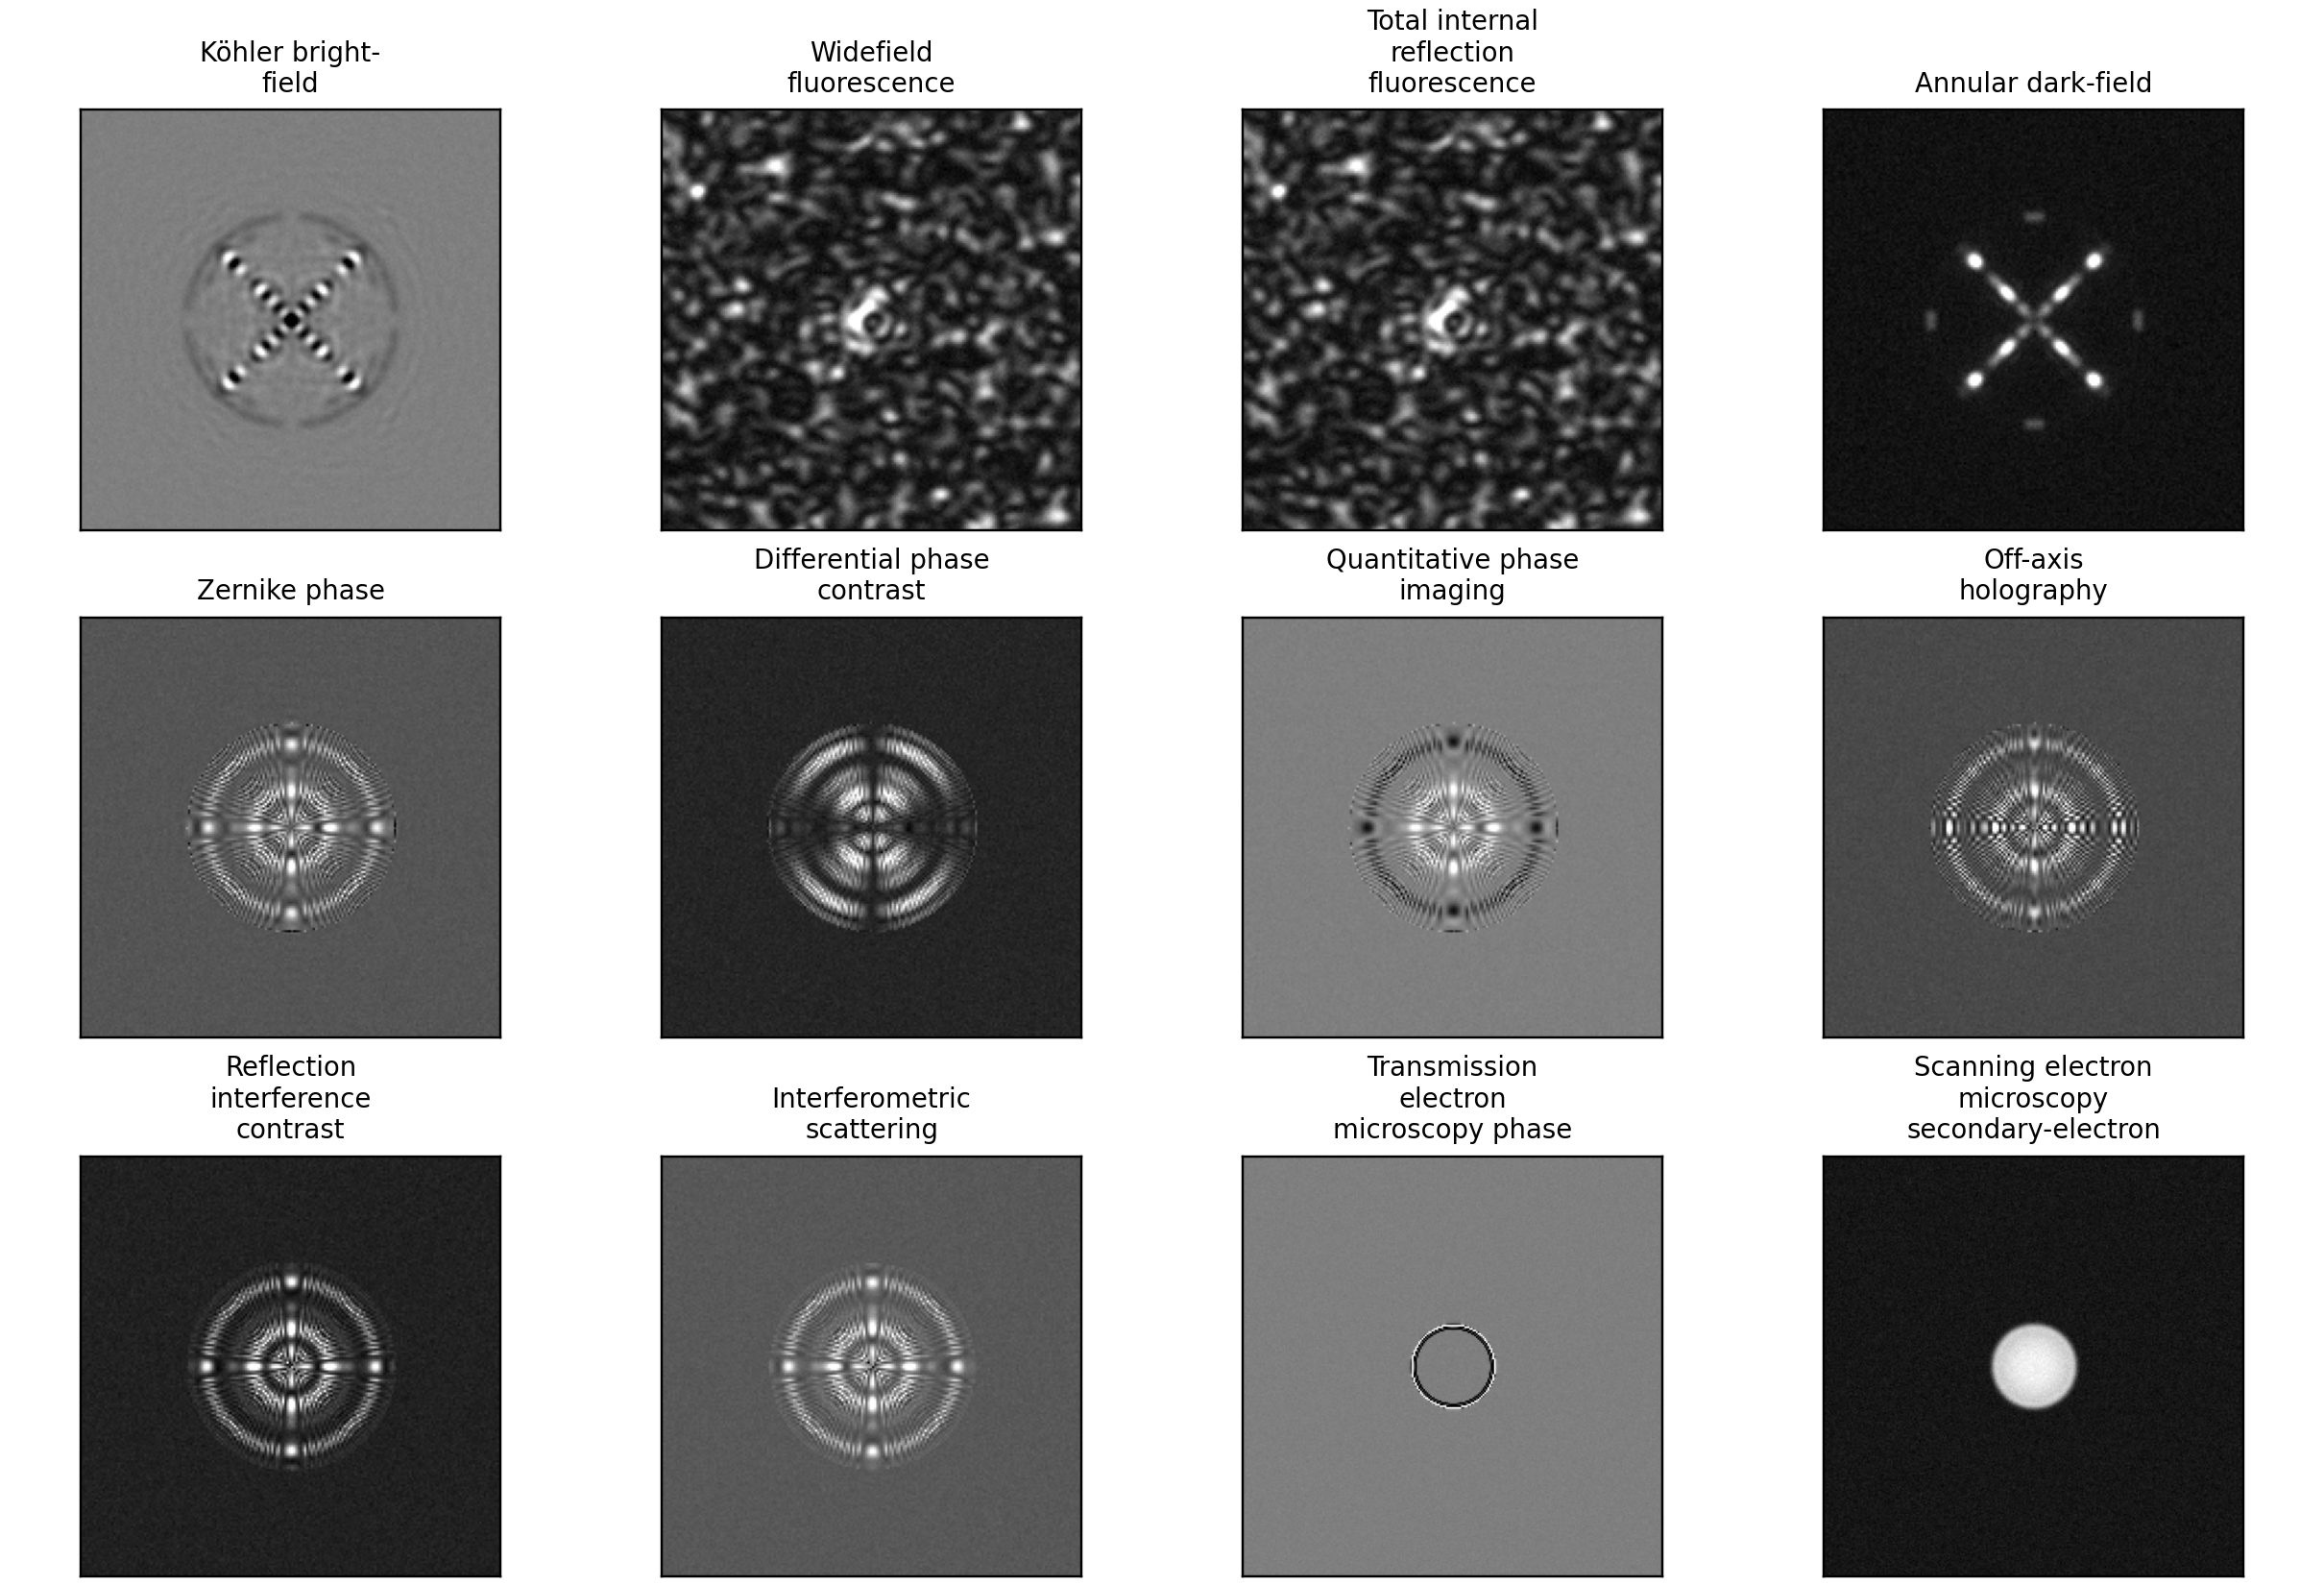
\includegraphics[width=\linewidth]{figures/imaging-modes.png}
\caption{Modality panel. The same latent particle state is rendered through the forward-modality panel on a common physical display field. Each panel is a camera-style windowed detector or phase display with an embedded scale bar; signed-contrast diagnostic arrays and resolved sampling metadata are saved separately for quantitative inspection.}
\label{fig:modality-panel}
\end{figure}
}{%
\generatedfallbackfigure{fig:modality-panel}{Modality panel. The same latent particle state is rendered through the forward-modality panel on a common physical display field.}{Required figure asset.}
}

\paragraph{Composite-particle rendering.} Composite particles are represented as rigid assemblies of primitive components --- spheres and non-spherical primitives such as ellipsoids and rods --- with body-frame offsets. The panel in \cref{fig:composite-gallery} shows representative rendered frames for a sphere, an ellipsoid, a rod (cylinder primitive), a dimer, a linear trimer, a bent triatomic, a bowtie-like assembly, and a tetrahedral 3D assembly under matched camera, imaging-model, and noise settings. The gallery includes non-spherical primitives so the rendered geometry is not restricted to isotropic spheres; compact assemblies can still project similarly, so orientation identifiability is quantified separately for the $\mathrm{SE}(3)$ diagnostic subset in \cref{tab:orientation-crlb}.

\IfFileExists{figures/composite-gallery.png}{%
\begin{figure}[H]
\centering
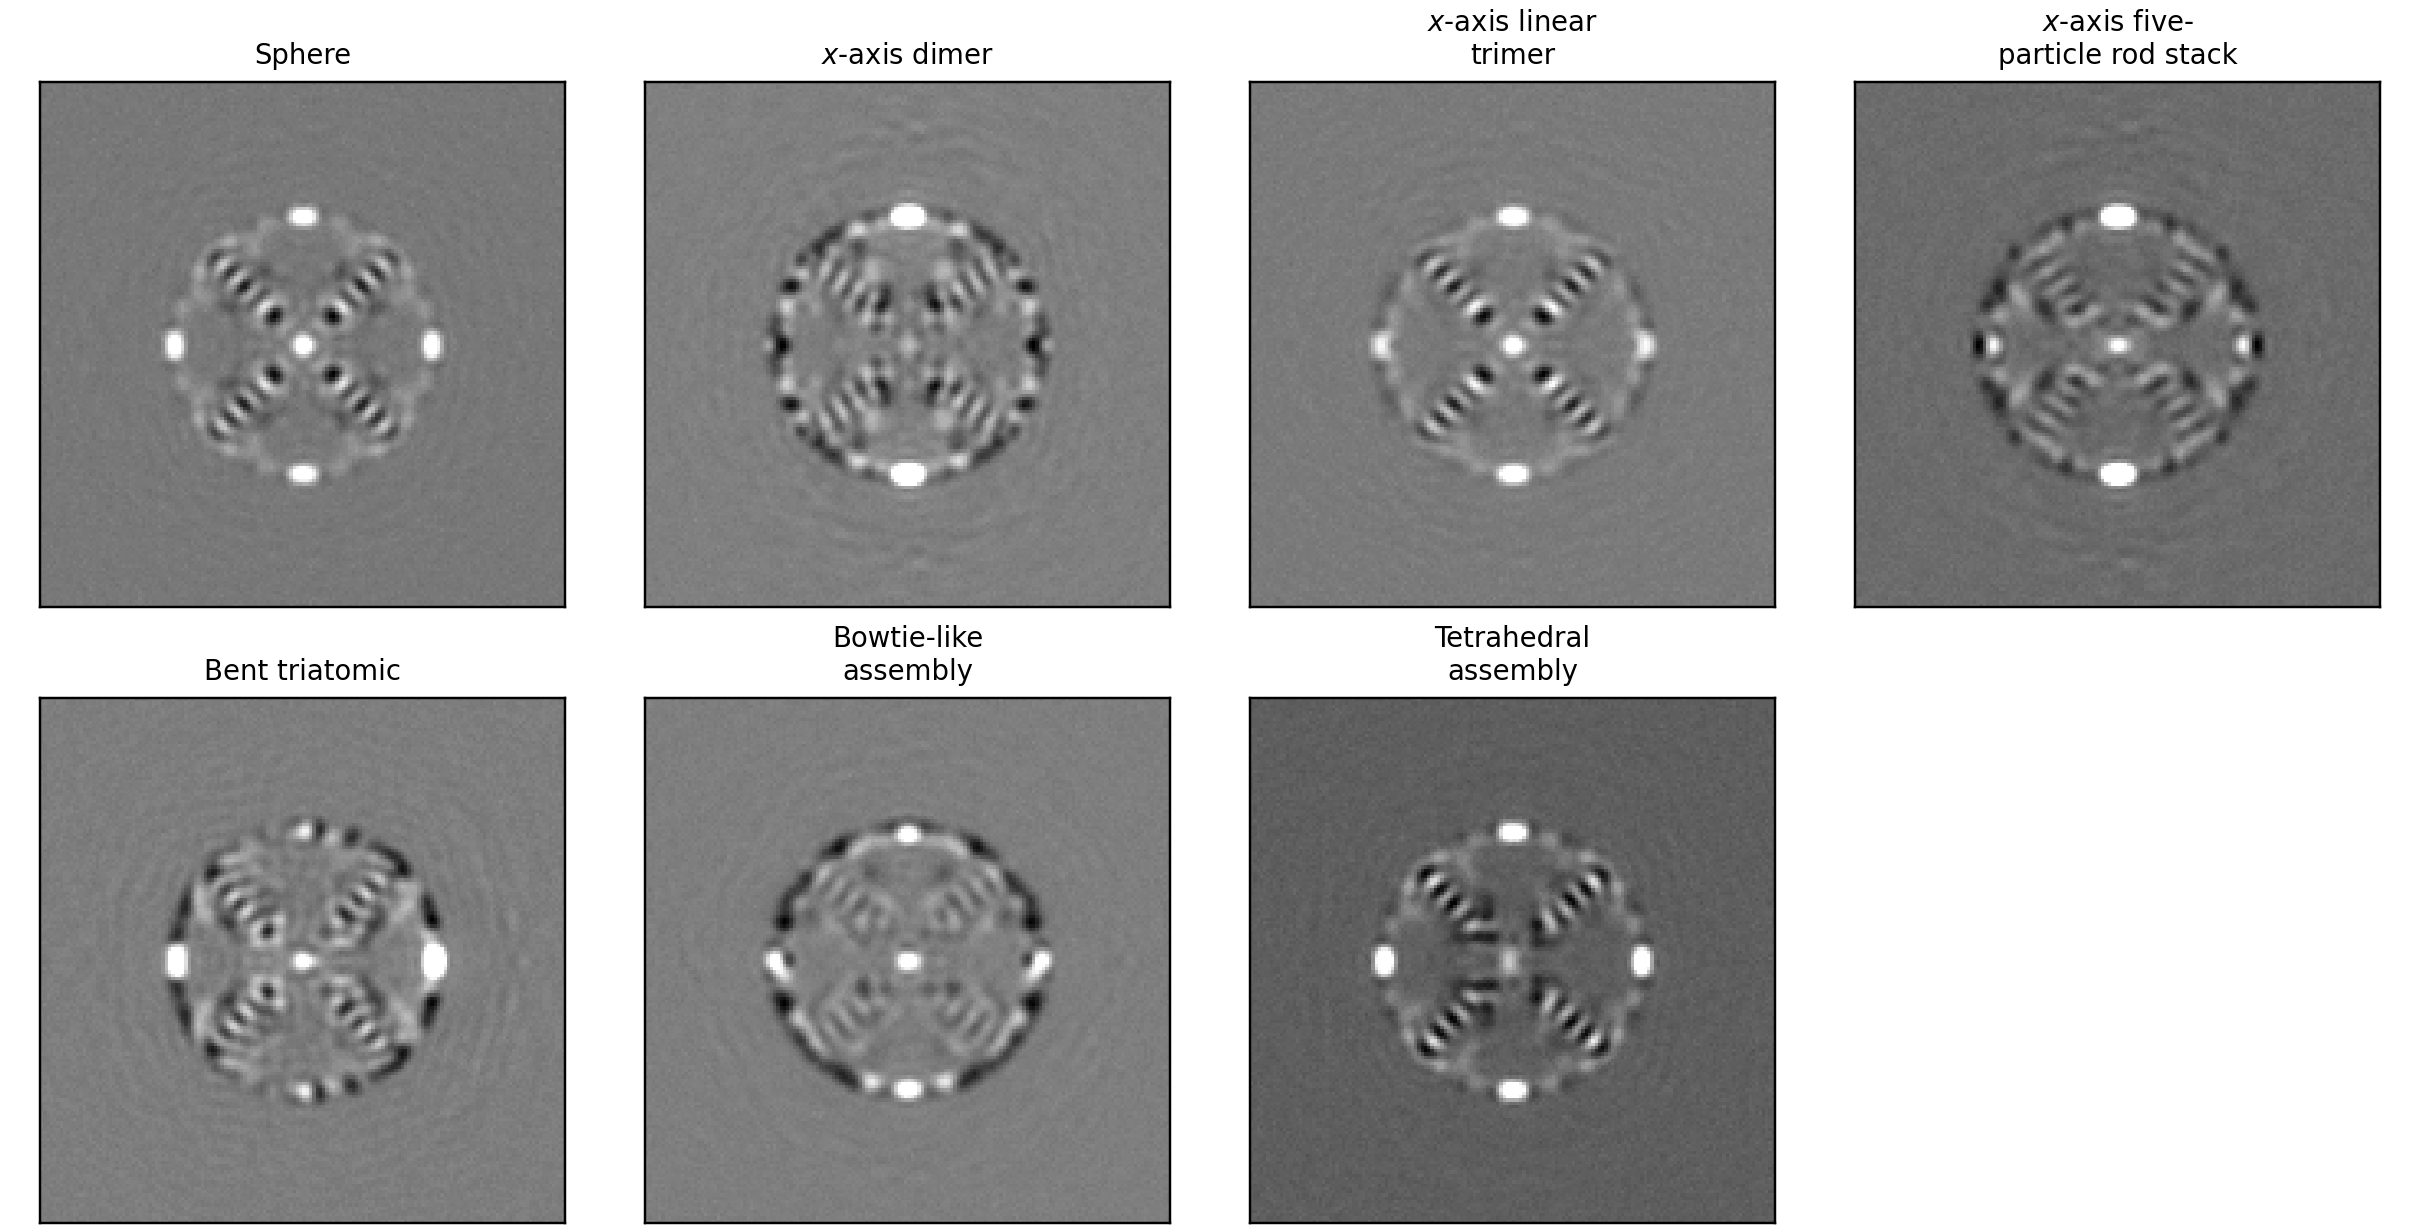
\includegraphics[width=\linewidth]{figures/composite-gallery.png}
\caption{Composite particle gallery. The displayed shapes are rendered under identical camera, imaging-model, and noise settings. Compact assemblies can project similarly in this display; \cref{tab:orientation-crlb} reports orientation-rank diagnostics for the subset used in the $\mathrm{SE}(3)$ check.}
\label{fig:composite-gallery}
\end{figure}
}{%
\generatedfallbackfigure{fig:composite-gallery}{Composite particle gallery. The displayed shapes are rendered under identical camera, imaging-model, and noise settings.}{Required figure asset.}
}

\paragraph{Coupled-cluster scattering.} For closely spaced components the independent-superposition model is not the right physical object, so Syniscopy partitions a particle's components into interaction clusters by exact inter-component surface gap and solves close clusters with a coupled solver (Section~\ref{sec:physical-model}). \Cref{tab:coupled-scattering-demo} demonstrates this on a dimer whose inter-component gap is swept: at large gap the coupled solver reproduces the independent superposition (the decoupling limit), and as the gap closes the coupled contrast and lateral Cram\'{e}r--Rao bound diverge from the superposition while the coupling-regime gate marks the uncoupled proxy invalid. This both validates the coupled solver against the decoupling limit and shows the regime where the uncoupled model would misstate the bound.

\IfFileExists{figures/coupled-scattering-demo-table.tex}{%
\begin{table}[H]
\centering
\small
\resizebox{\linewidth}{!}{\input{figures/coupled-scattering-demo-table}}
\caption{Coupled-cluster scattering demonstration on a dimer at decreasing inter-component surface gap. The coupled solver's contrast and lateral Cram\'{e}r--Rao bound are compared against the independent (uncoupled) superposition, alongside the cluster-partition coupling-regime gate. Large gaps recover the superposition (decoupling limit); small gaps diverge and the gate flags the uncoupled proxy as invalid.}
\label{tab:coupled-scattering-demo}
\end{table}
}{%
\generatedfallbacktable{tab:coupled-scattering-demo}{Coupled-cluster scattering demonstration: coupled vs uncoupled dimer contrast and Cram\'{e}r--Rao bound across inter-component gap, with the coupling-regime gate.}{Required table asset.}
}

\subsection{Cram\'{e}r--Rao and Fisher information diagnostics}

\paragraph{Theory-to-diagnostic map.}
Each formal statement in \cref{sec:information-layer} is paired with a simulator diagnostic in \cref{tab:theoretical-support}. The table lists, for each theorem, corollary, or operational diagnostic, the output used to inspect the corresponding behavior.

\IfFileExists{figures/theoretical-support-table.tex}{%
\begin{table}[H]
\centering
\small
\resizebox{\linewidth}{!}{\begin{tabular}{@{}>{\raggedright\arraybackslash}p{0.18\linewidth}>{\raggedright\arraybackslash}p{0.28\linewidth}>{\raggedright\arraybackslash}p{0.28\linewidth}>{\raggedright\arraybackslash}p{0.18\linewidth}@{}}
\toprule
Claim & What it says & Simulator diagnostic & Output shown in \\
\midrule
Symmetry rank theorem & Contrast-functional continuous symmetry predicts $\mathrm{SE}(3)$ rank deficit. & Rank predictor plus observed Fisher rank and singular-axis metadata. & Table~\ref{tab:orientation-crlb}. \\
Fusion-symmetry corollary & Fusion breaks only rotation symmetries not shared by each selected modality. & Fused-rank predictor from the intersection stabilizer dimension. & Tables~\ref{tab:orientation-crlb} and~\ref{tab:fusion-symmetry-diagnostic}. \\
Reject-rule support-score decomposition & Supported supervision uses bounded signal, information, temporal, and ambiguity support factors combined as clipped log odds by default. & Supervision consistency evaluation for representative supported, borderline, and excluded targets. & Table~\ref{tab:supervision-audit}. \\
Registration covariance & Registration uncertainty monotonically weakens fused information. & Registration-adjusted bound and degradation fraction. & Table~\ref{tab:registration-degradation}. \\
Loewner dominance & Loewner-dominated information-rate matrices can be pruned for fixed-budget scheduling. & Synthetic two-matrix dominance check and Loewner-maximal set. & Table~\ref{tab:loewner-dominance}. \\
Structured-background nuisance projection & Structured background removes the nuisance-subspace projection of signed particle derivatives. & Raw and nuisance-adjusted Fisher summaries for a synthetic background basis. & Table~\ref{tab:structured-background-loss}. \\
Detected-quanta scaling & Poisson-dominated detected-quanta scaling changes the Cram\'{e}r--Rao bound as $1/\sqrt{\alpha}$ when normalized image shape and detector regime are fixed. & Fixed-budget ordering and detected-quanta sweep. & Table~\ref{tab:budget-normalized}; Fig.~\ref{fig:detected-quanta-budget-pareto}. \\
Diminishing fusion returns & Best-$k$ fusion bounds can saturate under a supplied modality set. & Best-$k$ fusion curve under the implemented modality set. & Fig.~\ref{fig:fusion-curve}. \\
\bottomrule
\end{tabular}
}
\caption{How the theoretical contributions map to simulator diagnostics. Established mathematical tools are used where stated; the paper's contributions are the shared-scene Fisher information framing, the contrast-symmetry rank theorem and fusion corollary, the matched microscope-packet format, and the reject-rule support-score supervision decomposition as implemented diagnostics.}
\label{tab:theoretical-support}
\end{table}
}{%
\generatedfallbacktable{tab:theoretical-support}{How the theoretical contributions map to simulator diagnostics.}{Required table asset.}
}

\begin{table}[H]
\centering
\small
\begin{tabular}{p{0.26\linewidth}p{0.64\linewidth}}
\toprule
Parameter & Diagnostic profile value \\
\midrule
Particle & 100~nm gold sphere unless varied; the same particle material state is passed to every microscope, while each microscope's contrast modality supplies its own response and noise parameters \\
Image grid & Head-to-head modality contracts use a shared \(192\times192\) detector grid, 65~nm pixel pitch, 384 pupil samples, and \(2\times\) point-spread-function oversampling; native-regime source-use rows are separate source-specific cases \\
Optical medium/objective & water medium $n=1.33$; immersion $n=1.518$; profile-specific numerical aperture or probe scale \\
Wavelength & 532~nm profile unless a modality profile overrides it (vectorial Debye default; scalar paraxial selectable) \\
Derivative and singularity rules & lateral spectral band-limited derivatives with Nyquist/boundary diagnostics; axial planes at $z_0\pm200$~nm; $\mathrm{SE}(3)$ orientation perturbations of 0.03~rad; singular axes use a scale-relative Fisher eigenvalue tolerance of $10^{-12}$ \\
Noise and budget & propagated detector noise for configured-profile rankings; $N_Q=5\times10^4$ for budget-normalized Poisson/phase diagnostics \\
\bottomrule
\end{tabular}
\caption{Representative diagnostic profile conventions for the configured-profile Cram\'{e}r--Rao examples in this section. These values are not a calibration of any specific bench; absolute bounds depend on supplied amplitude, detector, shared sampling, and noise parameters.}
\label{tab:default-profile}
\end{table}

\paragraph{Closed-form scaling checks.} The lateral Cram\'{e}r--Rao implementation includes checks against three expected laws: $\sigma_{xy}\propto 1/\mathrm{SNR}$ at fixed point-spread-function width, $\sigma_{xy}\propto d^{-3}$ for a controlled Rayleigh-amplitude response, and diameter-independence at fixed signal-to-noise ratio \cite{thompson-larson-webb,ober-ram-ward,juffmann-iscat-cobri-crlb}. \Cref{tab:closed-form-scaling-checks} reports the fitted exponent or residual for each check. These are software consistency diagnostics under controlled inputs, not empirical validation of microscope performance. The Rayleigh row holds the image geometry and noise fixed while scaling contrast amplitude as $d^3$, so the Fisher bound should scale as $d^{-3}$. The fixed-SNR diameter-independence check is a renormalized control in which the signal amplitude is held fixed as diameter changes; both controls are separate from the particle-size sweep in \cref{fig:particle-size-sweep}, where modality-specific contrast amplitude and noise can vary with diameter while the head-to-head observation grid is held fixed.

\IfFileExists{figures/closed-form-scaling-check-table.tex}{%
\begin{table}[H]
\centering
\small
\resizebox{\linewidth}{!}{\begin{tabular}{p{0.22\linewidth}p{0.34\linewidth}rrp{0.22\linewidth}}
\toprule
Check & Input sweep/control & Expected exponent & Fitted exponent & Residual summary \\
\midrule
Detected-quanta/SNR scaling & native interfero\allowbreak{}metric scattering microscopy SNR proxy sqrt(N\_Q) sweep & $-1.000$ & -1.000 & 1.000000; max rel. residual 0.0013\% \\
Rayleigh interfero\allowbreak{}metric scattering microscopy diameter scaling & controlled Rayleigh-amplitude Fisher sweep & $-3.000$ & -3.000 & 1.0000; max rel. residual 0.00\% \\
Fixed-SNR diameter control & diameter label varied with contrast/noise arrays held fixed & $0.000$ & 0.000 & max rel. change 0.000\% \\
\bottomrule
\end{tabular}
}
\caption{Closed-form scaling checks for the Fisher implementation. The first row uses the native iSCAT detected-quanta sweep converted to the Poisson-limited signal-to-noise proxy $\sqrt{N_Q}$, the Rayleigh row uses a controlled fixed-geometry contrast-amplitude sweep, and the fixed-SNR row is the renormalized control in which contrast and noise arrays are held fixed.}
\label{tab:closed-form-scaling-checks}
\end{table}
}{}

\paragraph{Configured-profile lateral Cram\'{e}r--Rao diagnostic.} Microscopes are reported under the shared instrument configuration summarized in \cref{tab:default-profile}; generated profile-card artifacts, when present, provide the per-microscope backend-fidelity cards. This head-to-head diagnostic is the fixed-instrument special case: it holds detector sampling and optics fixed across the compared microscopes and lets the contrast modality, backend, material/source interpretation, and detector-noise/count settings define the comparison. A general cross-microscope comparison instead lets each microscope carry its own optics and detector configuration; \Cref{tab:cross-microscope-comparison} reports such a comparison, in which microscopes that share a contrast modality but differ in instrument configuration (for example numerical aperture, pixel pitch, or detected-quanta budget) receive distinct Cram\'{e}r--Rao bounds. That two same-modality microscopes are ranked separately, rather than collapsed into one modality row, is the property that makes the microscope --- not the bare modality --- the unit of comparison. The lateral derivative implementation is checked in \cref{tab:lateral-spectral-diagnostics}: the bound uses the single center-rendered contrast image and the exact spectral gradient, while the table reports whether the sampled image is sufficiently band-limited and contained in the field of view.

\IfFileExists{figures/cross-microscope-comparison-table.tex}{%
\begin{table}[H]
\centering
\small
\resizebox{\linewidth}{!}{\input{figures/cross-microscope-comparison-table}}
\caption{Cross-microscope comparison in which candidates that share a contrast modality differ in instrument configuration. Each row is a microscope; rows with the same modality but different numerical aperture, pixel pitch, or detected-quanta budget report distinct lateral Cram\'{e}r--Rao bounds, so they are ranked as separate candidates rather than merged into one modality entry. This is the general case for which the configured-profile table in \cref{tab:modality-ranking} is the fixed-instrument special case.}
\label{tab:cross-microscope-comparison}
\end{table}
}{%
\generatedfallbacktable{tab:cross-microscope-comparison}{Cross-microscope comparison: same-modality microscopes with differing instrument configuration receive distinct Cram\'{e}r--Rao bounds and are ranked as separate candidates.}{Required table asset.}
}

\paragraph{Comparison contracts.} Table-to-table claims are contract-specific in this section. We use four explicit contracts: Contract-LP (configured-profile lateral Cram\'{e}r--Rao), Contract-LZ (configured-profile axial/\(\mathrm{SE}(3)\) diagnostics), Contract-Q (detected-quanta-normalized comparison), and Contract-NR (native-regime source-use context). The same profile can therefore produce different orderings under different contracts.

Cram\'{e}r--Rao lower bounds in \Cref{tab:modality-ranking} are Contract-LP diagnostics over microscopes that share one instrument configuration: each row is a microscope reported on a shared physical coordinate frame with shared detector pitch and its own contrast-modality response/noise backend, not a native-instrument comparison. Because the instrument is held fixed, the table doubles as the fixed-instrument modality comparison. Bench mapping is approximate: the current configuration parameters do not absorb all stray light, alignment error, out-of-focus particles, dust, or detector nonlinearity; source-matching residuals are addressed explicitly through configurable sample-environment perturbations including \texttt{sample\_environment\_pattern\_roughness\_model}, \texttt{sample\_environment\_pattern\_roughness\_amplitude}, \texttt{sample\_environment\_pattern\_roughness\_correlation\_pixels}, \texttt{sample\_environment\_pattern\_roughness\_phase\_std}, and \texttt{sample\_environment\_pattern\_roughness\_source} (for \texttt{source\_matched} mode), with roughness-source coupling options \texttt{independent}, \texttt{coherent\_amplitude}, \texttt{field\_weighted}, \texttt{scene\_weighted}, and \texttt{channel\_weighted} (default: \texttt{channel\_weighted}). The transmission-electron-microscopy row uses its configured backend-specific dose and potential/contrast settings \texttt{ctf\_proxy}/\texttt{multislice\_lite}/\texttt{syniscopy\_multislice}; native transmission-electron-microscopy sampling remains a separate instrument-specific configuration in Contract-NR.

\Cref{tab:modality-ranking} reports the default Contract-LP configured-profile diagnostic bound and within-profile relative bound. Table~\ref{tab:lateral-spectral-diagnostics} reports the sampling and support diagnostics attached to the same lateral Fisher calculation, so Table~\ref{tab:modality-ranking} should be read as a status-tagged configured-profile diagnostic rather than a universal ranking independent of sampling and field containment. Under the spectral lateral calculation, the lowest lateral bounds are scanning electron microscopy secondary-electron, interferometric scattering microscopy, and off-axis digital holography in this configured profile; rows with large Nyquist-band energy or boundary energy should not be used for precise numerical claims without rerunning at an adequate field size and detector sampling. The differential-phase-contrast row is reported via the configured vectorial Debye asymmetric-illumination model: opposite half-disc condenser-source images are rendered, passed through shifted objective pupils, differenced, and normalized. Metadata records the selected DPC transfer model, illumination sigma, source sampling count, channel model, and vectorial detection mode; split-pupil/Foucault and phase-gradient proxy DPC are explicit alternate settings rather than the default row.

\IfFileExists{figures/modality-profile-card-table.tex}{%
\begin{table}[H]
\centering
\small
\resizebox{\linewidth}{!}{\begin{tabular}{p{0.18\linewidth}p{0.18\linewidth}p{0.17\linewidth}p{0.18\linewidth}p{0.15\linewidth}p{0.14\linewidth}}
\toprule
Modality & Profile/fidelity & Domain/units & Paper category & Validation & Scope \\
\midrule
partially coherent Köhler bright-field & vectorial\_abbe\_kohler\_bright\_field & contrast/relative\_reference & core\_scalar\_optical\_profile & unchecked & model-conditioned shared-scene diagnostic under the listed profile parameters \\
widefield fluorescence & vectorial\_photophysics\_fidelity\_based & count/detector\_count & core\_scalar\_optical\_profile & diagnostic only & model-conditioned shared-scene diagnostic under the listed profile parameters \\
total internal reflection fluorescence & vectorial\_photophysics\_fidelity\_based & count/detector\_count & core\_scalar\_optical\_profile & diagnostic only & model-conditioned shared-scene diagnostic under the listed profile parameters \\
annular Köhler dark-field & scalar\_abbe\_annular\_kohler\_dark\_field & count/detector\_count & core\_scalar\_optical\_profile & unchecked & model-conditioned shared-scene diagnostic under the listed profile parameters \\
Zernike phase contrast & model\_conditional\_profile & count/detector\_count & scalar\_proxy\_profile & unchecked & model-conditioned shared-scene diagnostic under the listed profile parameters \\
differential phase contrast & model\_conditional\_profile & count/detector\_count & scalar\_proxy\_profile & unchecked & model-conditioned shared-scene diagnostic under the listed profile parameters \\
quantitative phase imaging & model\_conditional\_profile & phase/radian & phase\_domain\_profile & unchecked & model-conditioned shared-scene diagnostic under the listed profile parameters \\
off-axis digital holography & model\_conditional\_profile & fringe\_count/detector\_count & scalar\_proxy\_profile & unchecked & model-conditioned shared-scene diagnostic under the listed profile parameters \\
reflection interference contrast microscopy & model\_conditional\_profile & contrast/relative\_reference & scalar\_proxy\_profile & unchecked & model-conditioned shared-scene diagnostic under the listed profile parameters \\
interfero\allowbreak{}metric scattering microscopy & model\_conditional\_profile & contrast/relative\_reference & core\_scalar\_optical\_profile & unchecked & model-conditioned shared-scene diagnostic under the listed profile parameters \\
transmission electron microscopy phase contrast & syniscopy\_multislice\_physics\_based & electron\_count/electron\_count & high\_fidelity\_electron\_profile & diagnostic only & model-conditioned shared-scene diagnostic under the listed profile parameters \\
scanning electron microscopy secondary-electron & syniscopy\_transport\_sem\_lite & electron\_count/electron\_count & high\_fidelity\_electron\_profile & diagnostic only & model-conditioned shared-scene diagnostic under the listed profile parameters \\
\bottomrule
\end{tabular}
}
\caption{Human-readable modality profile cards used by the configured-profile tables. Full machine-readable profile identifiers are retained in the generated artifact manifest and supplemental metadata.}
\label{tab:modality-profile-cards}
\end{table}
}{}

Total internal reflection fluorescence and widefield fluorescence are separate configured fluorescence profiles in \cref{tab:modality-ranking}. A separate native-regime source-use audit row for total internal reflection fluorescence exercises angle-derived evanescent excitation and trajectory depth; that audit row is not the configured-profile ranking row in \cref{tab:modality-ranking}.

Appendix~\ref{sec:source-use-audit} reports the native-regime source-use audit. That audit documents source use, source category, parameter-match status, computed localization scale where applicable, and source-reported scale. Only source categories that report or derive a localization scale populate the computed-localization column; dimensional-metrology and modality-principle rows are retained for provenance without being treated as particle-center localization checks. In particular, the native interferometric-scattering audit path uses the opt-in Fresnel-reference and high-numerical-aperture dipole-collection controls and gives a nanometer-scale result under that native check, whereas the configured-profile interferometric-scattering row belongs to the cross-modality diagnostic table.

The annular K\"{o}hler dark-field row is finite under the configured gold-particle scattering profile. Singular entries, when they occur, indicate that the selected diagnostic image provides no finite Fisher bound under that profile, not that experimental dark-field localization is impossible.

\IfFileExists{figures/modality-ranking-table.tex}{%
\begin{table}[H]
\centering
\small
\resizebox{\linewidth}{!}{\begin{tabular}{r p{0.26\linewidth} p{0.22\linewidth} r r p{0.16\linewidth}}
\toprule
Order & Modality & Profile/fidelity & $\sigma_{xy}$ (nm) & Relative $\sigma_{xy}$ & Status \\
\midrule
1 & Zernike phase contrast & model\_conditional\_profile & 0.013 & 1.000 & failed convergence \\
2 & interfero\allowbreak{}metric scattering microscopy & model\_conditional\_profile & 0.017 & 1.271 & failed convergence \\
3 & off-axis digital holography & model\_conditional\_profile & 0.042 & 3.209 & failed convergence \\
4 & scanning electron microscopy secondary-electron & syniscopy\_transport\_sem\_lite & 0.043 & 3.237 & failed convergence \\
5 & differential phase contrast & model\_conditional\_profile & 0.098 & 7.470 & failed convergence \\
6 & reflection interference contrast microscopy & model\_conditional\_profile & 0.150 & 11.41 & failed convergence \\
7 & quantitative phase imaging & model\_conditional\_profile & 1.290 & 98.08 & failed convergence \\
8 & transmission electron microscopy phase contrast & syniscopy\_multislice\_physics\_based & 1.879 & 142.9 & failed convergence \\
9 & partially coherent Köhler bright-field & vectorial\_abbe\_kohler\_bright\_field & 40.55 & 3084.1 & failed convergence \\
10 & annular Köhler dark-field & scalar\_abbe\_annular\_kohler\_dark\_field & 586.1 & 44576.6 & failed convergence \\
11 & total internal reflection fluorescence & vectorial\_photophysics\_fidelity\_based & 96359.5 & 7.329e+06 & failed convergence \\
12 & widefield fluorescence & vectorial\_photophysics\_fidelity\_based & 96398.0 & 7.331e+06 & failed convergence \\
\bottomrule
\end{tabular}
}
\caption{Default Contract-LP lateral Cram\'{e}r--Rao diagnostic values using the spectral band-limited lateral derivative. The table reports Syniscopy diagnostic values only and should not be read as a native-instrument benchmark independent of the sampling/support status; native-regime literature scale checks are separated into the source-use audit in Appendix~\ref{sec:source-use-audit}.}
\label{tab:modality-ranking}
\end{table}
}{%
\generatedfallbacktable{tab:modality-ranking}{Configured-profile lateral Cram\'{e}r--Rao ordering over the configured modality profiles.}{Required table asset.}
}

Lateral rows are no longer accepted or rejected by a finite-difference step sweep, because the lateral derivative has no perturbation step. Instead, \Cref{tab:lateral-spectral-diagnostics} reports the physical sampling/support diagnostics that determine whether the spectral derivative is trustworthy for the configured grid.

\IfFileExists{figures/lateral-spectral-diagnostics-table.tex}{%
\begin{table}[H]
\centering
\small
\resizebox{\linewidth}{!}{\input{figures/lateral-spectral-diagnostics-table}}
\caption{Lateral spectral-derivative sampling diagnostics for the configured-profile Cram\'{e}r--Rao diagnostic. The lateral Fisher matrix is computed from the exact FFT gradient of the center-rendered contrast image; the diagnostic columns report the derivative basis, Nyquist-band energy fraction, boundary energy fraction, numerical rank, and row status used to decide whether the sampled image is adequately band-limited and field-contained.}
\label{tab:lateral-spectral-diagnostics}
\end{table}
}{%
\generatedfallbacktable{tab:lateral-spectral-diagnostics}{Lateral spectral-derivative sampling diagnostics for the configured-profile Cram\'{e}r--Rao diagnostic.}{Required table asset.}
}

\paragraph{Partial-order comparison.} The scalar bound in \Cref{tab:modality-ranking} is one projection of the comparison, not the verdict. Because the central claim is that there is no universal ordering, the comparison is reported as a partial order. \Cref{tab:partial-order-comparison} gives two views over the same candidate set. The Loewner information order marks a candidate as information-dominated when another candidate's Fisher matrix is at least as large on every parameter direction ($F_A-F_B\succeq 0$); this is contract-independent and compares the information itself rather than a scalarization. The multi-criterion Pareto front is taken over localization precision together with the supplied acquisition-cost axes (dose, acquisition time, and a destructiveness flag); a candidate is dominated only when another is no worse on every axis and strictly better on at least one. Two candidates can therefore be genuinely incomparable --- one more precise, the other lower-dose or non-destructive --- and the front is the set of defensible choices rather than a single winner. The scalar rank is shown only as a reference projection.

\IfFileExists{figures/partial-order-comparison-table.tex}{%
\begin{table}[H]
\centering
\small
\resizebox{\linewidth}{!}{\input{figures/partial-order-comparison-table}}
\caption{Partial-order microscope comparison over the configured candidate set. Columns report whether each candidate is Loewner-information-maximal, whether it lies on the multi-criterion Pareto front over precision and the supplied acquisition-cost axes, the candidate(s) that dominate it when it is off the front, and its scalar rank as a reference projection. Candidates on the front are mutually incomparable defensible choices; a single scalar ranking would hide that.}
\label{tab:partial-order-comparison}
\end{table}
}{%
\generatedfallbacktable{tab:partial-order-comparison}{Partial-order microscope comparison: Loewner-information-maximal set and multi-criterion Pareto front over precision and acquisition-cost axes, with the scalar rank as a reference projection.}{Required table asset.}
}

\Cref{fig:particle-size-sweep} shows the corresponding particle-size sweep. Diameter-dependent contrast scaling can change the ordering, so the sweep should not be read as a universal modality ranking for every contract or as the fixed-SNR diameter-independence check above.

\IfFileExists{figures/particle-size-sweep.png}{%
\begin{figure}[H]
\centering
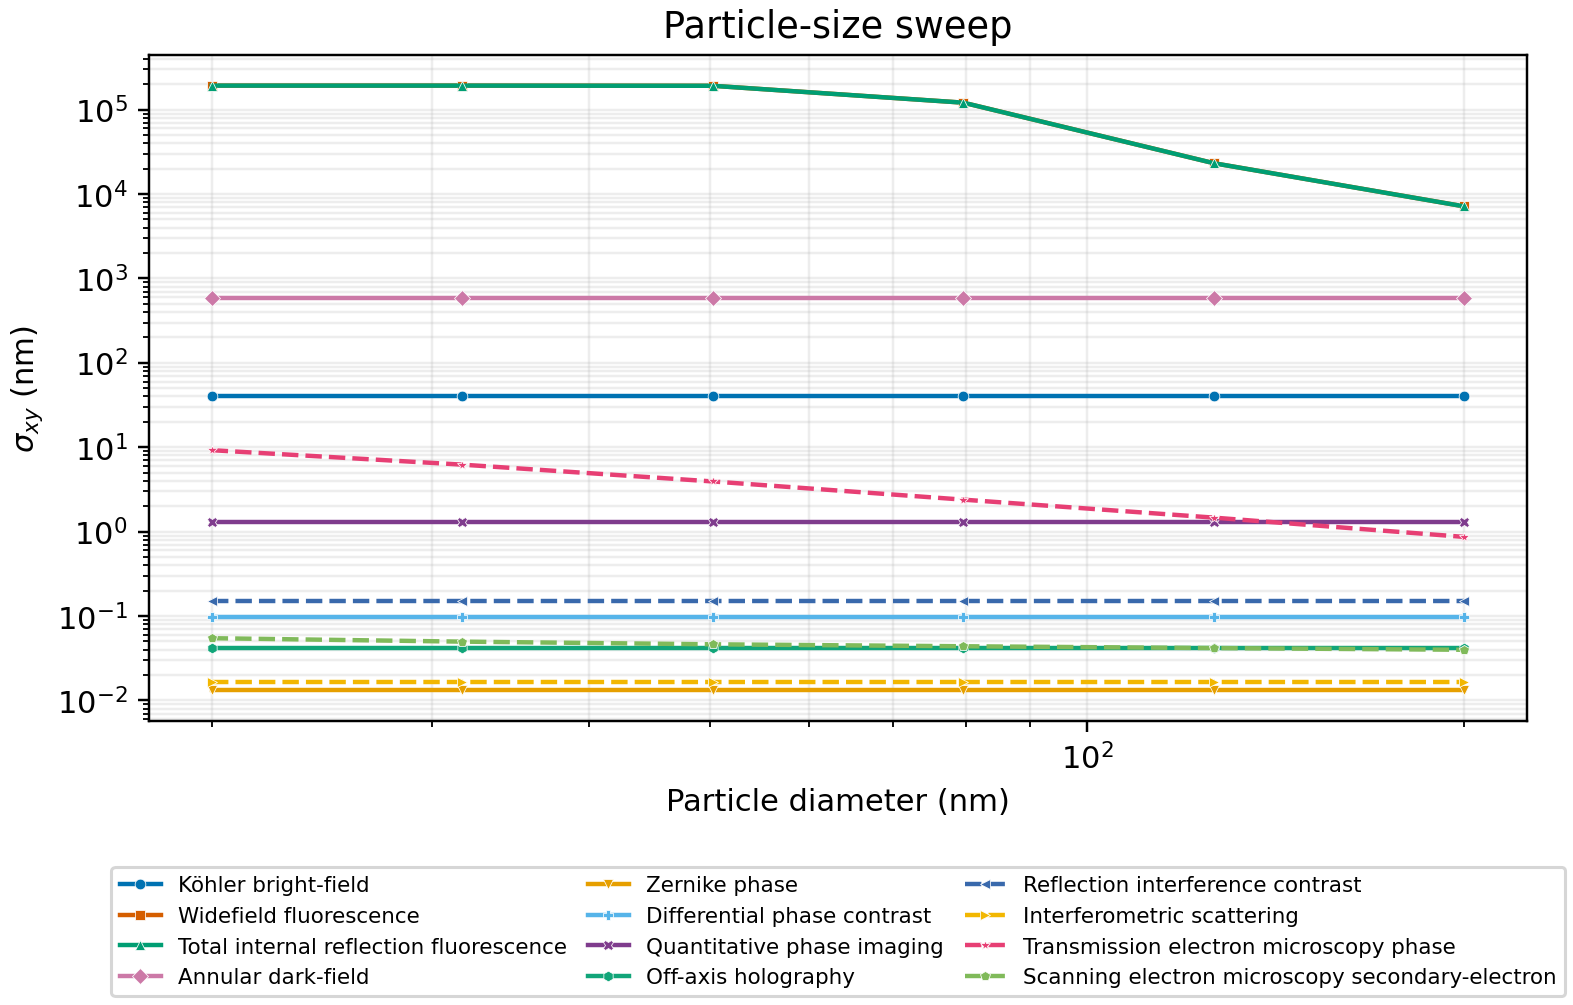
\includegraphics[width=0.85\linewidth]{figures/particle-size-sweep.png}
\caption{Particle-size sweep under the Contract-LP spectral lateral-derivative convention. Each color/marker/line-style combination is one imaging modality, identified by the legend below the axes. The curves expose how diameter-dependent contrast scaling can change modality diagnostics across particle sizes. Unless separately regenerated with per-diameter spectral sampling/support metadata, these curves inherit the configured-grid assumptions in Table~\ref{tab:lateral-spectral-diagnostics}; singular cases are treated as nonfinite rather than assigned artificial finite values.}
\label{fig:particle-size-sweep}
\end{figure}
}{%
\generatedfallbackfigure{fig:particle-size-sweep}{Particle-size sweep. The curves expose how diameter-dependent contrast scaling can change fixed-instrument candidate diagnostics across particle sizes. Singular cases are treated as nonfinite rather than assigned artificial finite values.}{Required figure asset.}
}

\paragraph{Axial and orientation bounds.} Contract-LZ uses a three-plane axial extension at $z_0-\Delta z$, $z_0$, and $z_0+\Delta z$, and reports default $\sigma_z$ values and singular rows in \cref{tab:axial-crlb}. The $\mathrm{SE}(3)$ extension uses one center render plus symmetric perturbation pairs for $z$, $\omega_x$, $\omega_y$, and $\omega_z$, where $\omega$ denotes an infinitesimal body-frame rotation. Symmetric composites report singular body axes explicitly in \cref{tab:orientation-crlb}. The diagnostic subset includes anisotropic primitives (a true rod and an ellipsoid) and a coupled cluster, so the reported continuous symmetries arise from intrinsic particle anisotropy rather than from the isotropy of spherical sub-components. Most finite axial rows in \Cref{tab:axial-crlb} fail the axial derivative-step convergence gate (Table~\ref{tab:axial-convergence-crlb}); widefield fluorescence, TEM phase contrast, and SEM remain singular under this Contract-LZ setup. Therefore this table is an axial singularity/diagnostic report, not a universal claim of native axial instrument performance.

\IfFileExists{figures/orientation-crlb-table.tex}{%
\begin{table}[H]
\centering
\small
\resizebox{\linewidth}{!}{\begin{tabular}{lcccccc}
\toprule
Particle & Numerical Fisher rank & Axis-estimability rank & Stabilizer $d$ & Null rotation axes $\ge d$ & Generic rank & Singular rotation axes \\
\midrule
Sphere & 3 & 3 & 3 & 3 & 3 & rotation about $x$, rotation about $y$, rotation about $z$ \\
$x$-axis dimer & 5 & 5 & 1 & 1 & 5 & bond-axis rotation \\
$x$-axis linear trimer & 5 & 5 & 1 & 1 & 5 & chain-axis rotation \\
Bent triatomic & 6 & 6 & 0 & 0 & 6 & none \\
$x$-axis five-particle rod stack & 5 & 5 & 1 & 1 & 5 & rod-axis rotation \\
Tetrahedral assembly & 6 & 6 & 0 & 0 & 6 & none \\
\bottomrule
\end{tabular}
}
\caption{$\mathrm{SE}(3)$ rank and singular-axis metadata by composite shape. The numerical Fisher rank is shown beside the axis-estimability rank, the rank predicted from continuous contrast symmetry, and the guaranteed number of null rotation axes; $\omega_x,\omega_y,\omega_z$ are infinitesimal body-frame rotations about the principal axes.}
\label{tab:orientation-crlb}
\end{table}
}{%
\generatedfallbacktable{tab:orientation-crlb}{$\mathrm{SE}(3)$ rank and singular-axis metadata by composite shape. The numerical Fisher rank and axis-estimability rank are shown beside the symmetry-predicted generic rank and the symmetry-guaranteed nullity lower bound.}{Required table asset.}
}

\IfFileExists{figures/orientation-spectrum-table.tex}{%
\begin{table}[H]
\centering
\small
\resizebox{\linewidth}{!}{\begin{tabular}{p{0.24\linewidth}rrrp{0.32\linewidth}}
\toprule
Particle & Numerical rank & Rank tol. & Cond. & Fisher eigenvalues \\
\midrule
Sphere & 3 & 2.213e-19 & 11.34 & 0.000000e+00;0.000000e+00;0.000000e+00;1.950746e-08;2.200424e-07;2.213089e-07 \\
$x$-axis dimer & 5 & 2.739e-12 & 9.605e+07 & -1.424544e-23;2.851051e-08;2.748695e-07;3.920763e-07;7.154251e-03;2.738545e+00 \\
$x$-axis linear trimer & 5 & 3.032e-12 & 2.207e+07 & -2.581085e-21;1.373882e-07;1.191681e-06;1.758532e-06;2.435891e-02;3.032129e+00 \\
Bent triatomic & 6 & 2.710e-12 & 1.915e+08 & 1.414638e-08;3.082185e-07;4.799763e-07;1.412055e-02;2.222073e-02;2.709711e+00 \\
$x$-axis five-particle rod stack & 5 & 6.759e-12 & 5.332e+07 & 5.870607e-22;1.267657e-07;6.826466e-07;1.706997e-06;1.061646e-01;6.758892e+00 \\
Tetrahedral assembly & 6 & 3.895e-12 & 8.709e+07 & 4.471888e-08;4.213445e-07;4.598425e-07;6.979435e-01;3.880060e+00;3.894585e+00 \\
\bottomrule
\end{tabular}
}
\caption{$\mathrm{SE}(3)$ Fisher spectrum metadata for the orientation-rank diagnostic. The table records the eigenvalue spectrum and rank tolerance used to declare singular axes.}
\label{tab:orientation-spectrum}
\end{table}
}{}

\IfFileExists{figures/orientation-rank-convergence-table.tex}{%
\begin{table}[H]
\centering
\small
\resizebox{\linewidth}{!}{\begin{tabular}{p{0.30\linewidth}p{0.23\linewidth}p{0.23\linewidth}c}
\toprule
Particle & Numerical ranks over $\delta\omega$ & Singular axes over $\delta\omega$ & Pass \\
\midrule
Sphere & 0.015:3; 0.030:3; 0.060:3 & 0.015:omega\_x, rotation about $y$, rotation about $z$, 0.030:omega\_x, rotation about $y$, rotation about $z$, 0.060:omega\_x, rotation about $y$, rotation about $z$ & yes \\
$x$-axis dimer & 0.015:5; 0.030:5; 0.060:5 & 0.015:omega\_x, 0.030:omega\_x, 0.060:omega\_x & yes \\
$x$-axis linear trimer & 0.015:5; 0.030:5; 0.060:5 & 0.015:omega\_x, 0.030:omega\_x, 0.060:omega\_x & yes \\
Bent triatomic & 0.015:6; 0.030:6; 0.060:6 & 0.015:none, 0.030:none, 0.060:none & yes \\
$x$-axis five-particle rod stack & 0.015:5; 0.030:5; 0.060:5 & 0.015:omega\_x, 0.030:omega\_x, 0.060:omega\_x & yes \\
Tetrahedral assembly & 0.015:6; 0.030:6; 0.060:6 & 0.015:none, 0.030:none, 0.060:none & yes \\
\bottomrule
\end{tabular}
}
\caption{$\mathrm{SE}(3)$ orientation-step convergence check. The numerical Fisher rank and singular-axis labels are recomputed across symmetric body-frame rotation perturbations and must remain stable for the diagnostic to pass.}
\label{tab:orientation-rank-convergence}
\end{table}
}{}

\Cref{tab:fusion-symmetry-diagnostic} records the cross-modality fusion-symmetry case on a single fixed particle geometry, separately from the per-shape table. The two fused entries are two modalities imaging the \emph{same} particle: one modality's contrast functional retains a continuous rotational symmetry that the other modality's contrast functional breaks --- the modality-induced regime in which the contrast-functional stabilizer differs from the geometric stabilizer. For example, a polarization-resolved vectorial modality breaks an axis that a polarization-blind scalar modality leaves as a rotational null. Their stabilizer intersection therefore has no continuous rotational symmetry, giving predicted fused rotational rank 3 and full $\mathrm{SE}(3)$ rank 6. This is the operational content of Corollary~\ref{cor:fusion-symmetry-breaking}: fusion recovers an axis when one modality's imaging physics breaks a symmetry the other retains, distinct from the particle geometry.

\IfFileExists{figures/fusion-symmetry-diagnostic-table.tex}{%
\begin{table}[H]
\centering
\small
\resizebox{\linewidth}{!}{\begin{tabular}{p{0.36\linewidth}p{0.18\linewidth}p{0.14\linewidth}p{0.14\linewidth}p{0.12\linewidth}}
\toprule
Diagnostic case & Stabilizer dims. & Intersection dim. & Rotational rank & $\mathrm{SE}(3)$ rank \\
\midrule
Axisymmetric contrast alone & $1$ & $1$ & $2$ & $5$ \\
Symmetry-breaking contrast alone & $0$ & $0$ & $3$ & $6$ \\
Fused subset & $1, 0$ & $0$ & $3$ & $6$ \\
\bottomrule
\end{tabular}
}
\caption{Fusion-symmetry diagnostic on a single fixed geometry. Two modalities image the same particle; the fused pair removes a rotational null that one modality retains, because the second modality's contrast functional --- not the particle geometry --- observes that axis. The connected stabilizer intersection is therefore trivial. This is the modality-induced case in which the contrast-functional stabilizer differs from the geometric stabilizer.}
\label{tab:fusion-symmetry-diagnostic}
\end{table}
}{}

\IfFileExists{figures/cross-modality-axial-table.tex}{%
\begin{table}[H]
\centering
\small
\resizebox{\linewidth}{!}{\begin{tabular}{r p{0.34\linewidth} p{0.30\linewidth} r r}
\toprule
Order & Modality & Profile/fidelity & $\sigma_z$ (nm) & Relative $\sigma_z$ \\
\midrule
1 & interfero\allowbreak{}metric scattering microscopy & model\_conditional\_profile & 0.085 & 1.000 \\
2 & differential phase contrast & model\_conditional\_profile & 0.300 & 3.536 \\
3 & Zernike phase contrast & model\_conditional\_profile & 0.558 & 6.577 \\
4 & off-axis digital holography & model\_conditional\_profile & 1.292 & 15.22 \\
5 & reflection interference contrast microscopy & model\_conditional\_profile & 2.632 & 31.01 \\
6 & quantitative phase imaging & model\_conditional\_profile & 14.73 & 173.5 \\
7 & partially coherent Köhler bright-field & vectorial\_abbe\_kohler\_bright\_field & 440.7 & 5192.2 \\
8 & annular Köhler dark-field & scalar\_abbe\_annular\_kohler\_dark\_field & 4099.5 & 48296.8 \\
9 & total internal reflection fluorescence & vectorial\_photophysics\_fidelity\_based & 94978.4 & 1.119e+06 \\
10 & widefield fluorescence & vectorial\_photophysics\_fidelity\_based & $\infty$ & $\infty$ \\
11 & transmission electron microscopy phase contrast & syniscopy\_multislice\_physics\_based & $\infty$ & $\infty$ \\
12 & scanning electron microscopy secondary-electron & syniscopy\_transport\_sem\_lite & $\infty$ & $\infty$ \\
\bottomrule
\end{tabular}
}
\caption{Default Contract-LZ axial Cram\'{e}r--Rao diagnostic and singularity report over the lateral-shared-profile setup. Infinite rows indicate no finite three-plane axial Fisher bound under the Contract-LZ diagnostic response; finite rows must be interpreted with the convergence states in Table~\ref{tab:axial-convergence-crlb}.}
\label{tab:axial-crlb}
\end{table}
}{%
\generatedfallbacktable{tab:axial-crlb}{Contract-LZ axial Cram\'{e}r--Rao ordering over the configured modality profiles.}{Required table asset.}
}

\IfFileExists{figures/axial-convergence-crlb-table.tex}{%
\begin{table}[H]
\centering
\small
\resizebox{\linewidth}{!}{\begin{tabular}{p{0.30\linewidth}p{0.22\linewidth}p{0.16\linewidth}p{0.14\linewidth}p{0.16\linewidth}}
\toprule
Modality & $\sigma_z$ over $\Delta z$ & Rank/order range & Span & Status \\
\midrule
partially coherent Köhler bright-field & 100.0:45.53; 200.0:440.7; 400.0:500.0 & 3 & 998.14\% & failed convergence \\
widefield fluorescence & 100.0:$\infty$; 200.0:$\infty$; 400.0:$\infty$ & 2 & -- & stable singular \\
total internal reflection fluorescence & 100.0:65229.3; 200.0:94978.4; 400.0:1.667e+05 & 3 & 155.55\% & failed convergence \\
annular Köhler dark-field & 100.0:4037.6; 200.0:4099.5; 400.0:4311.0 & 3 & 6.77\% & finite converged \\
Zernike phase contrast & 100.0:0.095; 200.0:0.558; 400.0:0.619 & 3 & 554.15\% & failed convergence \\
differential phase contrast & 100.0:0.151; 200.0:0.300; 400.0:0.364 & 3 & 140.94\% & failed convergence \\
quantitative phase imaging & 100.0:6.637; 200.0:14.73; 400.0:15.72 & 3 & 136.83\% & failed convergence \\
off-axis digital holography & 100.0:0.160; 200.0:1.292; 400.0:1.414 & 3 & 786.39\% & failed convergence \\
reflection interference contrast microscopy & 100.0:0.302; 200.0:2.632; 400.0:2.758 & 3 & 814.02\% & failed convergence \\
interfero\allowbreak{}metric scattering microscopy & 100.0:0.081; 200.0:0.085; 400.0:0.123 & 3 & 52.32\% & failed convergence \\
transmission electron microscopy phase contrast & 100.0:$\infty$; 200.0:$\infty$; 400.0:$\infty$ & 2 & -- & stable singular \\
scanning electron microscopy secondary-electron & 100.0:$\infty$; 200.0:$\infty$; 400.0:$\infty$ & 2 & -- & stable singular \\
\bottomrule
\end{tabular}
}
\caption{Contract-LZ axial derivative-step convergence check. The three-plane Fisher calculation is repeated across symmetric axial perturbations. Status values distinguish finite-converged rows, stable-singular rows with no finite axial bound under this diagnostic, and failed-convergence rows whose finite $\sigma_z$ values are not step-span validated.}
\label{tab:axial-convergence-crlb}
\end{table}
}{}

The axial table should be interpreted through the convergence gate: stable singular rows identify absent axial information under this diagnostic setup, while finite rows that fail the span criterion should not be used as precise axial performance claims.

\paragraph{Detected-quanta normalization.} Contract-Q assigns each count-domain modality the same detected-quanta budget and evaluates the resulting count image with a Poisson-Gaussian mean-Fisher diagnostic. The Contract-Q lateral Fisher derivative uses the same step-free spectral basis as Contract-LP, so its status metadata is a sampling/support diagnostic rather than a derivative-step convergence export. This is a common-budget diagnostic, not a claim that photons, electrons, reference-arm counts, and sample damage constraints are interchangeable operating costs. Quantitative phase imaging remains phase-domain and is evaluated through the phase-noise model, so its row is model-conditional rather than an intrinsic statement about all phase-imaging instruments. Because several count-domain rows in \Cref{tab:detected-quanta-normalization-metadata} have readout fractions materially away from zero (including 0.424 and 0.567), this scaling check is interpreted as a diagnostic reference rather than an exact model for every point in the reported sweep. \Cref{tab:budget-normalized} summarizes the fixed-budget comparison, and \cref{fig:detected-quanta-budget-pareto} shows the sweep over detected-quanta budgets. Contract-LP and Contract-Q answer different questions: the former uses propagated detector noise under representative modality profiles, while the latter maps eligible modalities to a fixed detected-quanta budget and Poisson/phase noise model. Signed-contrast and reference-arm modalities can move between these normalizations when a small contrast rides on a bright Poisson background. Dose, bleaching, radiation damage, heating, preparation, and destruction penalties belong to the acquisition-cost metadata layer and can be included when that contract is configured.

\IfFileExists{figures/detected-quanta-normalized-table.tex}{%
\begin{table}[H]
\centering
\small
\resizebox{\linewidth}{!}{\begin{tabular}{r p{0.26\linewidth} p{0.22\linewidth} r r p{0.16\linewidth}}
\toprule
Order & Modality & Profile/fidelity & $\sigma_{xy}$ (nm) & Relative $\sigma_{xy}$ & Status \\
\midrule
1 & interfero\allowbreak{}metric scattering microscopy & model\_conditional\_profile & 0.700 & 1.000 & failed convergence \\
2 & scanning electron microscopy secondary-electron & syniscopy\_transport\_sem\_lite & 1.152 & 1.645 & failed convergence \\
3 & differential phase contrast & model\_conditional\_profile & 2.992 & 4.273 & failed convergence \\
4 & off-axis digital holography & model\_conditional\_profile & 7.604 & 10.86 & failed convergence \\
5 & Zernike phase contrast & model\_conditional\_profile & 10.59 & 15.13 & failed convergence \\
6 & reflection interference contrast microscopy & model\_conditional\_profile & 12.00 & 17.15 & failed convergence \\
7 & total internal reflection fluorescence & vectorial\_photophysics\_fidelity\_based & 17.96 & 25.65 & failed convergence \\
8 & quantitative phase imaging & model\_conditional\_profile & 18.45 & 26.36 & failed convergence \\
9 & widefield fluorescence & vectorial\_photophysics\_fidelity\_based & 79.71 & 113.9 & failed convergence \\
10 & transmission electron microscopy phase contrast & syniscopy\_multislice\_physics\_based & 150.4 & 214.8 & failed convergence \\
11 & annular Köhler dark-field & scalar\_abbe\_annular\_kohler\_dark\_field & 1414.8 & 2021.0 & failed convergence \\
12 & partially coherent Köhler bright-field & vectorial\_abbe\_kohler\_bright\_field & 5619.3 & 8026.9 & failed convergence \\
\bottomrule
\end{tabular}
}
 \caption{Detected-quanta-budget-normalized lateral Cram\'{e}r--Rao bound at $N_Q=5\times10^4$ for Contract-Q. This common-budget diagnostic is not a native operating-regime ranking and is status-tagged by the spectral lateral sampling/support metadata in the current source outputs.}
\label{tab:budget-normalized}
\end{table}
}{%
\generatedfallbacktable{tab:budget-normalized}{Detected-quanta-budget-normalized lateral Cram\'{e}r--Rao bound at $N_Q=5\times10^4$.}{Required table asset.}
}

\IfFileExists{figures/detected-quanta-normalization-metadata-table.tex}{%
\begin{table}[H]
\centering
\small
\resizebox{\linewidth}{!}{\begin{tabular}{p{0.23\linewidth}p{0.15\linewidth}p{0.20\linewidth}p{0.18\linewidth}rr}
\toprule
Modality & Model & Count mean source & Derivative target & Scale & Readout frac. \\
\midrule
partially coherent Köhler bright-field & count & rendered\_detector\_counts & signed\_contrast\_scaled & 4.521e-05 & 0.424 \\
widefield fluorescence & count & rendered\_detector\_counts & signed\_contrast\_scaled & 1322.4 & 0.424 \\
total internal reflection fluorescence & count & rendered\_detector\_counts & signed\_contrast\_scaled & 6010.2 & 0.424 \\
annular Köhler dark-field & count & rendered\_detector\_counts & signed\_contrast\_scaled & 0.136 & 0.424 \\
Zernike phase contrast & count & rendered\_detector\_counts & signed\_contrast\_scaled & 1.348e-06 & 0.424 \\
differential phase contrast & count & rendered\_detector\_counts & signed\_contrast\_scaled & 1.058e-03 & 0.424 \\
quantitative phase imaging & phase & phase\_noise\_model & signed\_contrast\_scaled & -- & 0 \\
off-axis digital holography & count & rendered\_detector\_counts & signed\_contrast\_scaled & 2.696e-05 & 0.424 \\
reflection interference contrast microscopy & count & rendered\_detector\_counts & signed\_contrast\_scaled & 1.208e-04 & 0.424 \\
interfero\allowbreak{}metric scattering microscopy & count & rendered\_detector\_counts & signed\_contrast\_scaled & 1.171e-04 & 0.424 \\
transmission electron microscopy phase contrast & count & electron\_dose\_proxy & signed\_contrast\_scaled & 1.356e-04 & 0.424 \\
scanning electron microscopy secondary-electron & count & electron\_dose\_proxy & signed\_contrast\_scaled & 1.499e-03 & 0.567 \\
\bottomrule
\end{tabular}
}
\caption{Detected-quanta normalization metadata. Count-domain rows record the exposure scale and additive-readout fraction; phase-domain rows record the phase-variance path. Signed contrast remains the derivative target while the detector-count image supplies the Poisson mean. Ideal count-domain $F\propto N_Q$ scaling is exact only when additive readout variance is negligible.}
\label{tab:detected-quanta-normalization-metadata}
\end{table}
}{}

\IfFileExists{figures/detected-quanta-spectral-diagnostics-table.tex}{%
\begin{table}[H]
\centering
\small
\resizebox{\linewidth}{!}{\input{figures/detected-quanta-spectral-diagnostics-table}}
\caption{Contract-Q lateral spectral-derivative sampling diagnostics for detected-quanta-normalized ranking.}
\label{tab:detected-quanta-spectral-diagnostics}
\end{table}
}{\generatedfallbacktable{tab:detected-quanta-spectral-diagnostics}{Contract-Q lateral spectral-derivative sampling diagnostics for detected-quanta normalization.}{Required table asset.}}

\IfFileExists{figures/detected-quanta-budget-pareto.png}{%
\begin{figure}[H]
\centering
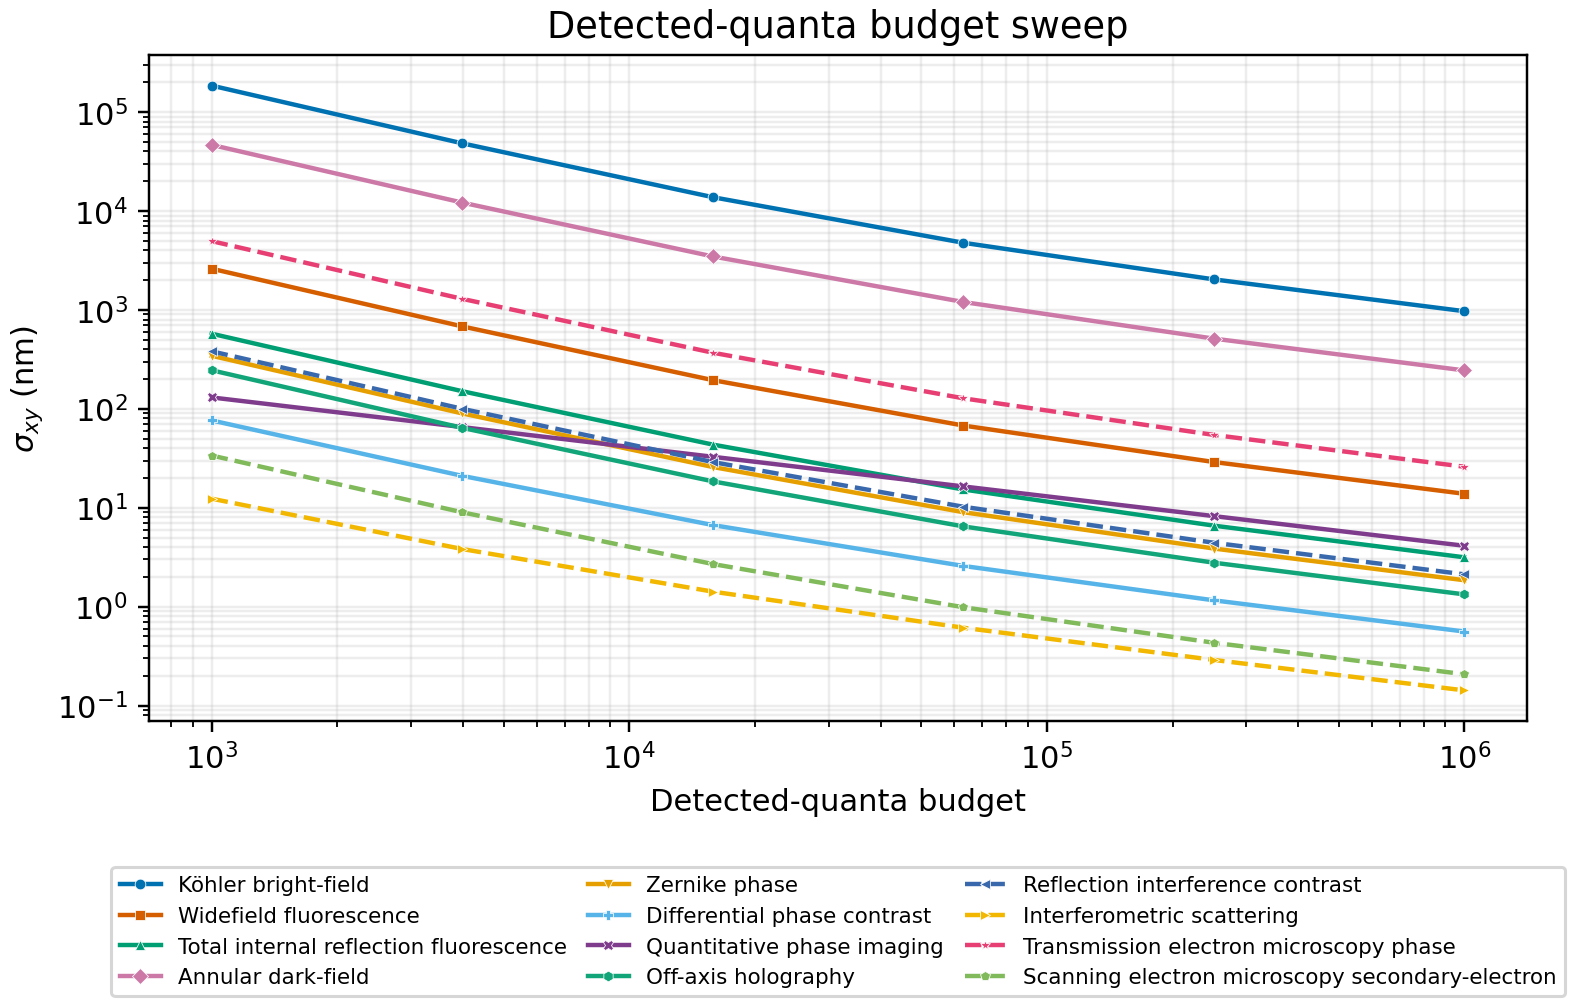
\includegraphics[width=0.85\linewidth]{figures/detected-quanta-budget-pareto.png}
\caption{Detected-quanta-budget sweep for Contract-Q. Each color/marker/line-style combination is one imaging modality, identified by the legend below the axes. Sweeping the plotted budget range within this configured profile shows whether the diagnostic ordering is stable or budget-dependent there. The plotted curves are accompanied by the Contract-Q spectral sampling diagnostics in Table~\ref{tab:detected-quanta-spectral-diagnostics}; singular budget cases are treated as nonfinite rather than assigned artificial finite values.}
\label{fig:detected-quanta-budget-pareto}
\end{figure}
}{%
\generatedfallbackfigure{fig:detected-quanta-budget-pareto}{Detected-quanta-budget sweep. Sweeping the plotted budget range within this configured profile shows whether the ordering is stable or budget-dependent there. Singular budget cases are treated as nonfinite rather than assigned artificial finite values.}{Required figure asset.}
}

\paragraph{Fusion Cram\'{e}r--Rao bound.} Best-$k$ subset search reports the lowest-bound single microscope candidate, the lowest-bound subset at each size, and full-library fusion in \cref{tab:fusion-crlb,fig:fusion-curve}. For these reported curves, Contract-LP is the underlying modality contract unless explicitly stated; each fused subset inherits the spectral lateral sampling/support status of its parent candidates from Table~\ref{tab:lateral-spectral-diagnostics}. The fusion bound is monotonically non-increasing with subset size under independent noise Fisher additivity. A lateral registration covariance can be supplied to model subpixel cross-channel alignment error before summing Fisher matrices; \cref{tab:registration-degradation} reports the corresponding synthetic degradation check. The full-library row is an algebraic independent-channel diagnostic, not a proposed physically simultaneous instrument. In experimental design, users should only fuse candidate microscopes whose physical channels are independently acquired, mutually compatible with the same sample state, and not alternate reconstructions of the same detected quanta.

\IfFileExists{figures/modality-fusion-crlb-table.tex}{%
\begin{table}[H]
\centering
\small
\resizebox{\linewidth}{!}{\begin{tabular}{r p{0.43\linewidth} r r p{0.20\linewidth}}
\toprule
$k$ & Modalities used & Fusion $\sigma_{xy}$ (nm) & Precision gain ($\sigma_{xy}^{(1)}/\sigma_{xy}^{(k)}$) & Interpretation \\
\midrule
1 & Zernike phase contrast & 0.013 & 1.000 & physically\_feasible\_fusion \\
2 & Zernike phase contrast, interferometric scattering microscopy & 0.010 & 1.273 & physically\_feasible\_fusion \\
3 & Zernike phase contrast, off-axis digital holography, interferometric scattering microscopy & 0.010 & 1.311 & physically\_feasible\_fusion \\
4 & Zernike phase contrast, off-axis digital holography, interferometric scattering microscopy, scanning electron microscopy secondary-electron & 9.760e-03 & 1.347 & algebraic\_diagnostic\_only \\
5 & Zernike phase contrast, differential phase contrast, off-axis digital holography, interferometric scattering microscopy, scanning electron microscopy secondary-electron & 9.712e-03 & 1.354 & algebraic\_diagnostic\_only \\
6 & Zernike phase contrast, differential phase contrast, off-axis digital holography, reflection interference contrast microscopy, interferometric scattering microscopy, scanning electron microscopy secondary-electron & 9.692e-03 & 1.357 & algebraic\_diagnostic\_only \\
7 & Zernike phase contrast, differential phase contrast, quantitative phase imaging, off-axis digital holography, reflection interference contrast microscopy, interferometric scattering microscopy, scanning electron microscopy secondary-electron & 9.691e-03 & 1.357 & algebraic\_diagnostic\_only \\
8 & Zernike phase contrast, differential phase contrast, quantitative phase imaging, off-axis digital holography, reflection interference contrast microscopy, interferometric scattering microscopy, transmission electron microscopy phase contrast, scanning electron microscopy secondary-electron & 9.691e-03 & 1.357 & algebraic\_diagnostic\_only \\
9 & partially coherent Köhler bright-field, Zernike phase contrast, differential phase contrast, quantitative phase imaging, off-axis digital holography, reflection interference contrast microscopy, interferometric scattering microscopy, transmission electron microscopy phase contrast, scanning electron microscopy secondary-electron & 9.691e-03 & 1.357 & algebraic\_diagnostic\_only \\
10 & partially coherent Köhler bright-field, annular Köhler dark-field, Zernike phase contrast, differential phase contrast, quantitative phase imaging, off-axis digital holography, reflection interference contrast microscopy, interferometric scattering microscopy, transmission electron microscopy phase contrast, scanning electron microscopy secondary-electron & 9.691e-03 & 1.357 & algebraic\_diagnostic\_only \\
11 & partially coherent Köhler bright-field, widefield fluorescence, annular Köhler dark-field, Zernike phase contrast, differential phase contrast, quantitative phase imaging, off-axis digital holography, reflection interference contrast microscopy, interferometric scattering microscopy, transmission electron microscopy phase contrast, scanning electron microscopy secondary-electron & 9.691e-03 & 1.357 & algebraic\_diagnostic\_only \\
12 & all 12 implemented modalities & 9.691e-03 & 1.357 & algebraic\_diagnostic\_only \\
\bottomrule
\end{tabular}
 and %% Generated by assemble-no-figures script
\endinput
}
\caption{Best-$k$ fusion Cram\'{e}r--Rao bound over the configured microscope candidates. Rows are selected by lowest fused $\sigma_{xy}$ under the algebraic independent-channel search and inherit the Contract-LP spectral sampling/support status of their parent candidates. The fused subsets should not be read as physically simultaneous instrument designs unless the selected channels have independent acquisition budgets, calibrated registration, and sample compatibility.}
\label{tab:fusion-crlb}
\end{table}
}{%
\generatedfallbacktable{tab:fusion-crlb}{Best-$k$ fusion Cram\'{e}r--Rao bound over the configured microscope candidates.}{Required table asset.}
}

\IfFileExists{figures/modality-fusion-crlb.png}{%
\begin{figure}[H]
\centering
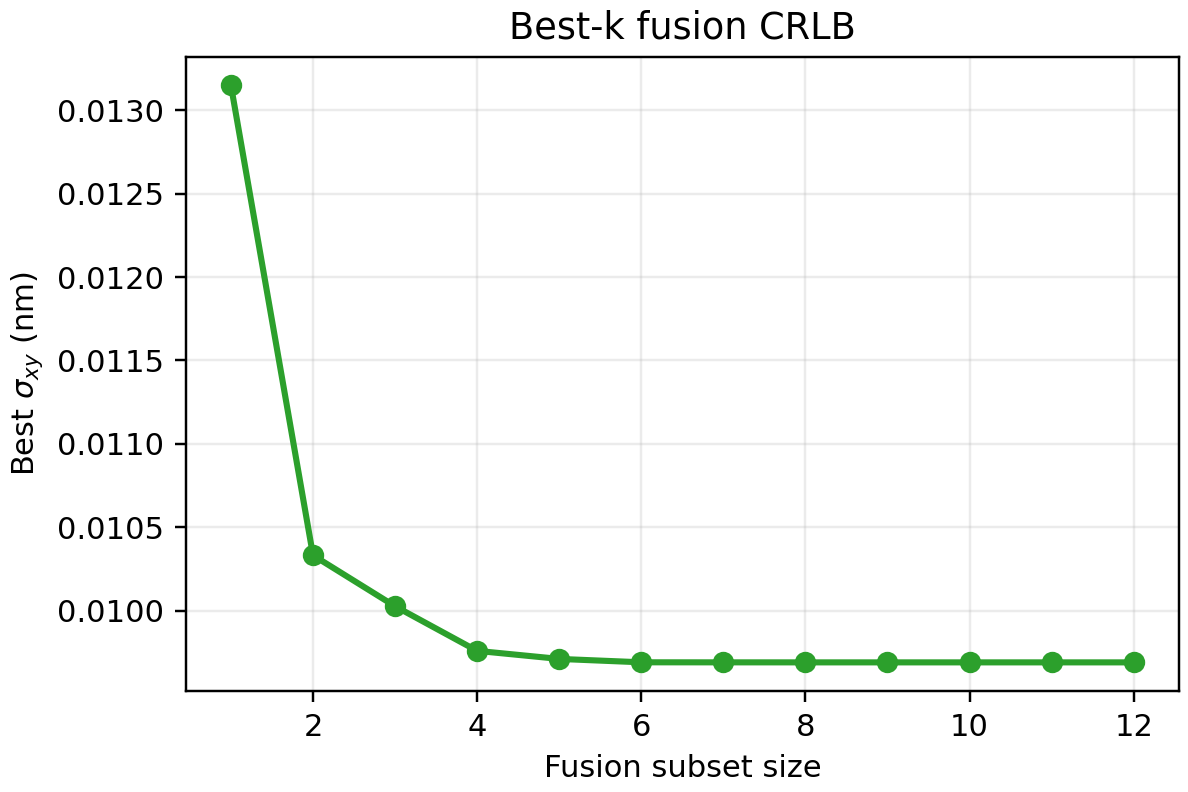
\includegraphics[width=0.85\linewidth]{figures/modality-fusion-crlb.png}
\caption{Fusion Cram\'{e}r--Rao bound versus subset size. Monotonicity follows from independent noise Fisher additivity. Under this profile, most of the lateral information is already captured by the first few selected microscope candidates; the curve inherits the Contract-LP spectral sampling/support status of its selected parent candidates.}
\label{fig:fusion-curve}
\end{figure}
}{%
\generatedfallbackfigure{fig:fusion-curve}{Fusion Cram\'{e}r--Rao bound versus subset size. The lowest attainable lateral bound is non-increasing as independent candidate Fisher matrices are added.}{Required figure asset.}
}

\IfFileExists{figures/fusion-independence-metadata-table.tex}{%
\begin{table}[H]
\centering
\small
\resizebox{\linewidth}{!}{\begin{tabular}{rp{0.36\linewidth}p{0.22\linewidth}p{0.20\linewidth}c}
\toprule
$k$ & Modalities & Physical status & Interpretation & Needs physical design review? \\
\midrule
1 & Zernike phase contrast & physically\_feasible\_sequential\_or\_simultaneous & physically\_feasible\_fusion & no \\
2 & Zernike phase contrast, interfero\allowbreak{}metric scattering microscopy & physically\_feasible\_sequential\_or\_simultaneous & physically\_feasible\_fusion & no \\
3 & Zernike phase contrast, off-axis digital holography, interfero\allowbreak{}metric scattering microscopy & physically\_feasible\_sequential\_or\_simultaneous & physically\_feasible\_fusion & no \\
4 & Zernike phase contrast, off-axis digital holography, interfero\allowbreak{}metric scattering microscopy, scanning electron microscopy secondary-electron & incompatible\_hard\_stop & algebraic\_diagnostic\_only & yes \\
12 & all 12 implemented modalities & incompatible\_hard\_stop & algebraic\_diagnostic\_only & yes \\
\bottomrule
\end{tabular}
}
\caption{Fusion-independence metadata emitted with representative best-$k$ subsets. The last column answers whether the subset still needs physical design review before interpreting the algebraic Fisher sum as an experimental acquisition.}
\label{tab:fusion-independence-metadata}
\end{table}
}{}

The lowest-bound $k$-subset curve saturates after the selected microscope candidates under this diagnostic profile because the leading scanning-electron, off-axis-holography, and interferometric-scattering terms already account for most of the lateral Fisher contribution in the configured profiles. The flat tail is profile-specific; it does not imply that large candidate libraries are generally redundant.

This serial-allocation solution is a boundary solution under fixed per-frame equal costs and the configured profiles; it inherits the Contract-LP spectral sampling/support status of the parent rows in Table~\ref{tab:lateral-spectral-diagnostics}. It should not be interpreted as a recommendation to replace optical live-particle workflows with SEM or other modalities, because practical compatibility, vacuum, dose, sample preparation, and field-of-view constraints are outside this synthetic objective model.

\IfFileExists{figures/time-allocation-crlb-table.tex}{%
\begin{table}[H]
\centering
\small
\resizebox{\linewidth}{!}{\begin{tabular}{l p{0.30\linewidth} r r r p{0.14\linewidth} p{0.16\linewidth}}
\toprule
Criterion & Nonzero allocation & $\sigma_{xy}$ (nm) & Gain vs. uniform & Gain vs. best single & Status & Termination \\
\midrule
A & zernike\_phase\_contrast:1 & 0.013 & 6.519 & 1.000 & invalid & no\_descent\_direction \\
D & zernike\_phase\_contrast:1 & 0.013 & 42.50 & 1.000 & invalid & no\_descent\_direction \\
E & zernike\_phase\_contrast:1 & 0.013 & 6.572 & 1.000 & invalid & no\_descent\_direction \\
\bottomrule
\end{tabular}
}
\caption{Serial time-allocation Cram\'{e}r--Rao diagnostic over the configured microscopes. Each row solves the fixed-time allocation problem for the stated A-, D-, or E-optimal scalarization using the same per-microscope Fisher matrices as the lateral Contract-LP diagnostic and therefore inherits their spectral sampling/support status. The allocation column reports nonzero time fractions under a unit total-time budget and equal per-frame time costs.}
\label{tab:time-allocation-crlb}
\end{table}
}{}

\IfFileExists{figures/registration-degradation-table.tex}{%
\begin{table}[H]
\centering
\small
\resizebox{\linewidth}{!}{\begin{tabular}{r r r r}
\toprule
Registration covariance diagonal (diagnostic coordinate units$^2$) & Fusion $\sigma_{xy}$ (nm) & Fusion gain & Degradation \\
\midrule
$0.00$ & $0.671$ & $1.139$ & $0.0\%$ \\
$0.01$ & $0.680$ & $1.122$ & $1.4\%$ \\
$0.10$ & $0.759$ & $1.006$ & $13.2\%$ \\
\bottomrule
\end{tabular}
}
\caption{Registration-covariance degradation diagnostic. Increasing residual cross-channel alignment covariance monotonically weakens the fused bound for the named modality subset. The diagnostic inherits the Contract-LP spectral sampling/support status of the fused modalities; the covariance entries are in nm$^2$ on the shared lateral $x/y$ parameter block.}
\label{tab:registration-degradation}
\end{table}
}{}

\paragraph{Per-pixel Fisher density.} The Cram\'{e}r--Rao implementation computes the per-pixel Fisher information integrand rather than only its spatial sum. The maps in \cref{fig:fisher-density-panel} localize the detector pixels with high Fisher contribution for the plotted modality profiles and can serve as optional information-aware training targets when a downstream model is configured for that auxiliary target.

\IfFileExists{figures/fisher-density-panel.png}{%
\begin{figure}[H]
\centering
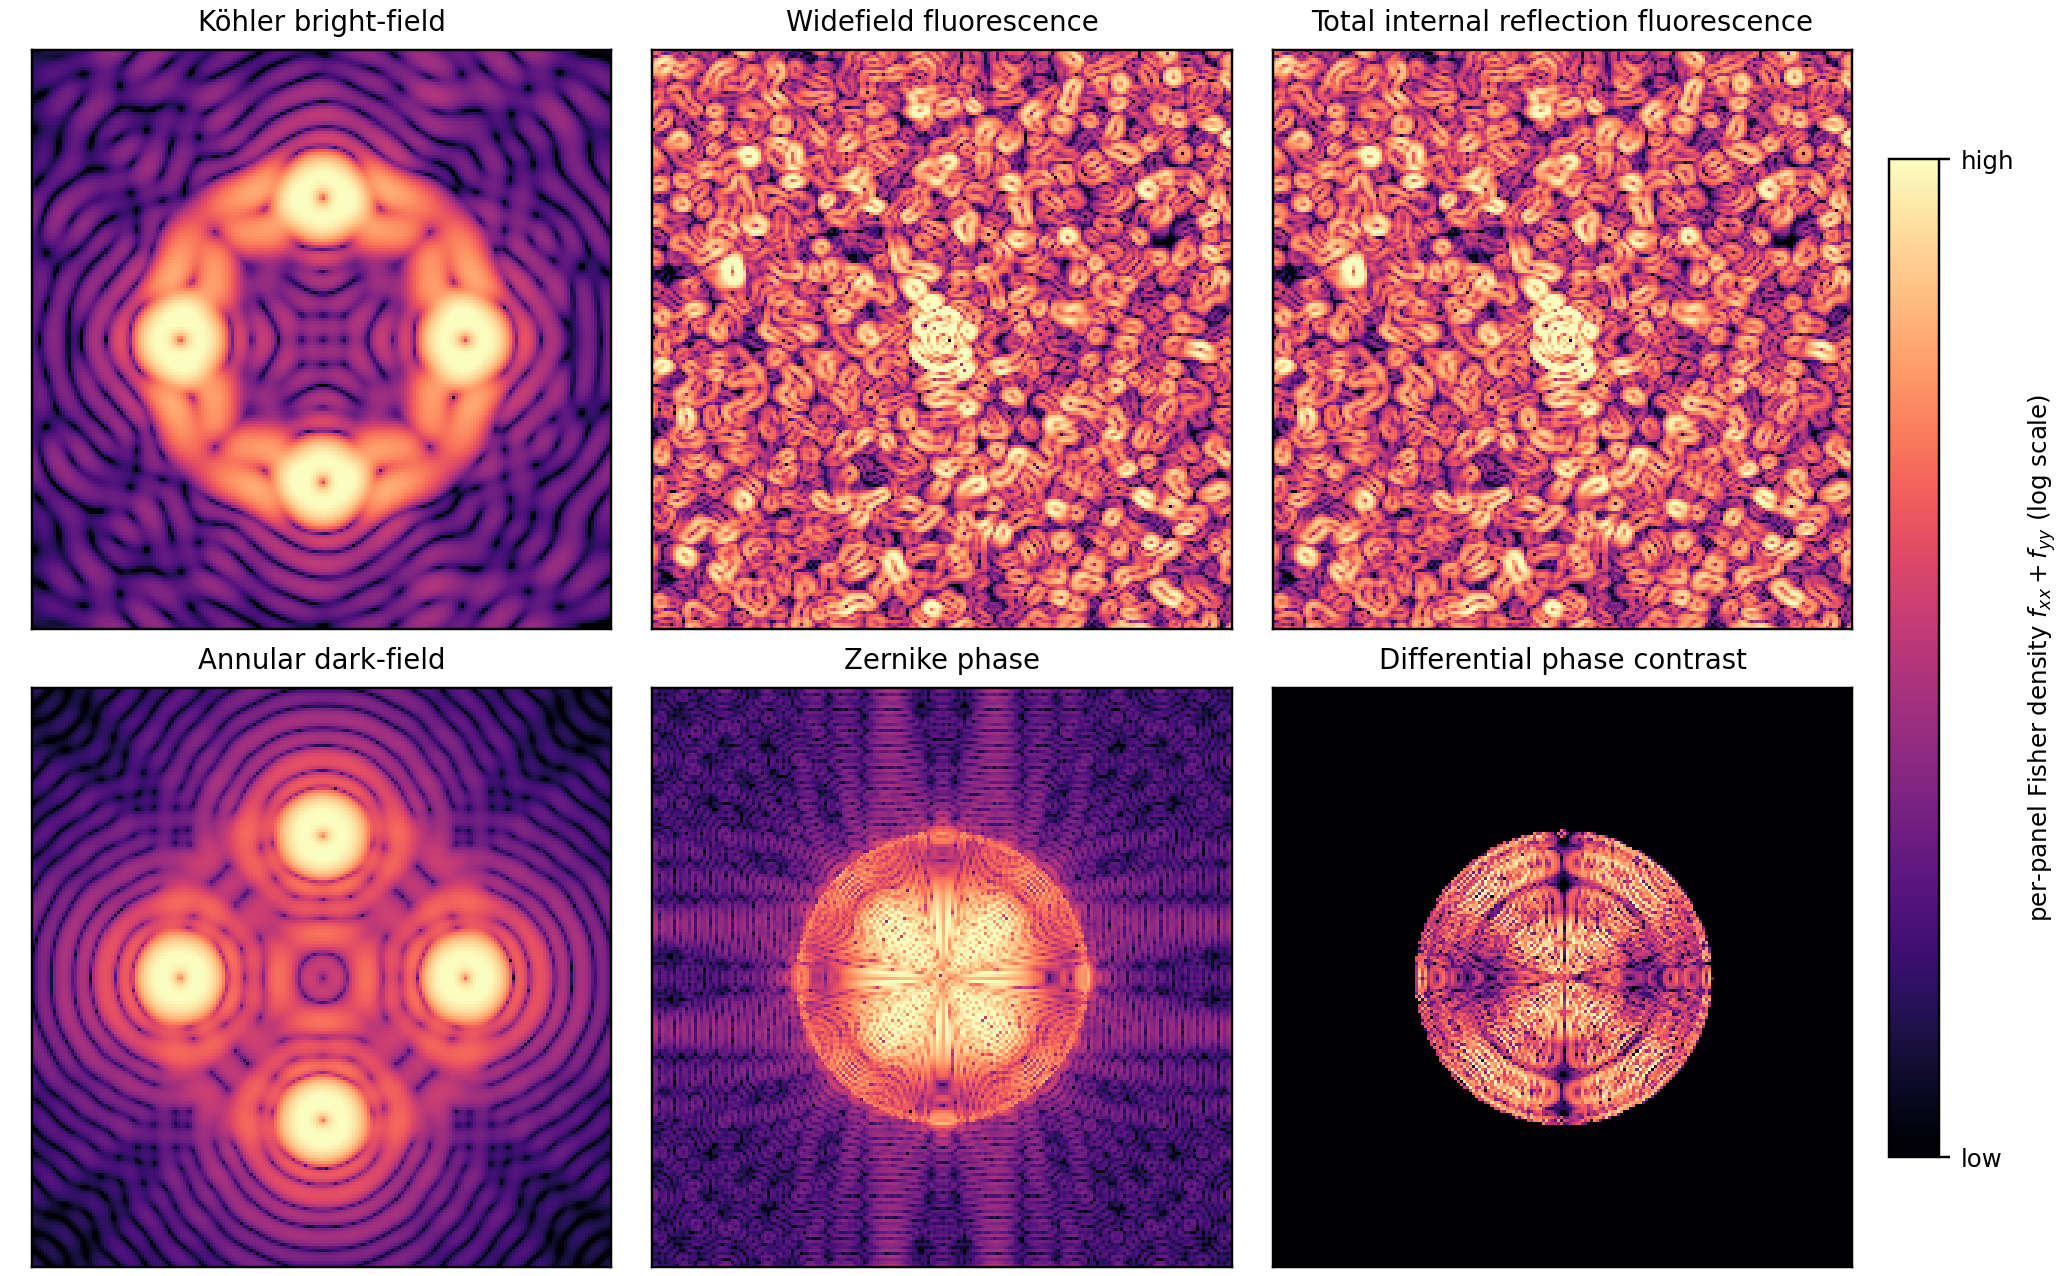
\includegraphics[width=\linewidth]{figures/fisher-density-panel.png}
\caption{Per-pixel Fisher information density maps. Each panel visualizes $f_{xx}+f_{yy}$ for one modality profile on the same particle. Each panel is independently log-scaled and percentile-clipped; the magma colorbar runs from dark (low) to bright (high) per-pixel Fisher density, and carries only that direction rather than a shared absolute scale.}
\label{fig:fisher-density-panel}
\end{figure}
}{%
\generatedfallbackfigure{fig:fisher-density-panel}{Per-pixel Fisher information density maps. Each panel visualizes $f_{xx}+f_{yy}$ for one modality profile on the same particle.}{Required figure asset.}
}

\paragraph{Implementation consistency diagnostics.} The following deterministic diagnostics are software consistency checks for the implemented Fisher and supervision layers. They verify expected algebraic behavior under controlled synthetic inputs; they are not empirical validation of microscope performance.

\Cref{tab:loewner-dominance} isolates the fixed-budget Loewner-dominance diagnostic with a two-matrix synthetic example.

\IfFileExists{figures/loewner-dominance-summary-table.tex}{%
\begin{table}[H]
\centering
\small
\resizebox{\linewidth}{!}{\begin{tabular}{p{0.20\linewidth}p{0.28\linewidth}p{0.16\linewidth}p{0.28\linewidth}}
\toprule
Pair & Information-rate test & Min. eigenvalue & Allocation effect \\
\midrule
A vs. B & $A_{A}-A_{B}\succeq 0$ & $2.0$ & keep A \\
B vs. A & $A_{B}-A_{A}\not\succeq 0$ & $-3.0$ & prune B if no minimum allocation is required \\
\bottomrule
\end{tabular}
}
\caption{Fixed-budget scheduling diagnostic. The table is a synthetic two-matrix check illustrating Loewner dominance, not a pair of real microscope modalities.}
\label{tab:loewner-dominance}
\end{table}
}{}

\Cref{tab:structured-background-loss} reports the structured-background nuisance projection diagnostic used to check that signed derivative maps, rather than squared information-density maps, are used for Schur-complement information loss.

\IfFileExists{figures/structured-background-loss-table.tex}{%
\begin{table}[H]
\centering
\small
\begin{tabular}{lccc}
\toprule
Diagnostic state & $F_{xx}$ & $F_{yy}$ & Mean loss over $x,y$ \\
\midrule
Raw particle derivatives & $50.0$ & $50.0$ & -- \\
After linear-$x$ nuisance projection & $0.0$ & $50.0$ & $50\%$ \\
\bottomrule
\end{tabular}

\caption{Structured-background nuisance projection diagnostic. The output is computed from signed lateral derivative maps for the named modality profile, noise-weighted inner products, and Schur-complement projection against the listed nuisance basis maps.}
\label{tab:structured-background-loss}
\end{table}
}{}

\subsection{Measurement-supported supervision}

The supervision consistency evaluation in \cref{tab:supervision-audit} evaluates deterministic particle-frame cases spanning supported, borderline, and singular zero-contrast targets without depending on Segment Anything Model 2. This deterministic evaluation set is not a population estimate for the full training corpus; it tests whether positive object pixels remain supervised while unsupported known-object pixels are routed to the ignore mask rather than silently converted to background.

\IfFileExists{figures/supervision-audit-table.tex}{%
\begin{table}[H]
\centering
\small
\begin{tabular}{p{0.40\linewidth}p{0.22\linewidth}p{0.28\linewidth}}
\toprule
Metric & Value & Check \\
\midrule
Particle-frame cases & 3 & deterministic evaluation set \\
Positive supervision pixel fraction & 33.3\% & supported target supervised \\
Ignored known-object pixels & 66.7\% & unsupported pixels ignored \\
Ignored particle fraction & 66.7\% & object-level support gate \\
Low-signal particle fraction & 66.7\% & signal factor \\
High-bound particle fraction & 66.7\% & information factor \\
Fisher-singular fraction & 33.3\% & singular-bound handling \\
Supported records & 1 & supported-case count \\

\end{tabular}
\caption{Supervision-schema consistency evaluation on a deterministic particle-frame set. Count rows are integers; support and exclusion rows are fractions of the deterministic evaluation set.}
\label{tab:supervision-audit}
\end{table}
}{%
\generatedfallbacktable{tab:supervision-audit}{Supervision-schema consistency evaluation on a deterministic particle-frame set.}{Required table asset.}
}

The deterministic supervision audit is the paper-facing supervision result. It verifies the simulator-side mask contract without promoting any downstream model-training run, checkpoint, or real-video transfer example to manuscript evidence.

\section{Scope and configured boundaries}
\label{sec:discussion}

\subsection{Configured forward-model scope}

The coherent-optical default is vectorial Debye, with explicit scalar paraxial and other fidelity knobs available through backend selectors when configured. Fresnel-reference and high-numerical-aperture dipole-collection controls are opt-in features used by the native interferometric scattering microscopy reference-check profile. The vectorial fluorescence backend includes a vectorial point-spread-function hook, directional bright-to-dark and dark-to-bright state kinetics, spectral scaling, bleaching controls, and detector-domain photon/electron/count propagation; proxy fluorescence modes remain selectable for lightweight diagnostics. Gibson--Lanni-style coverslip mismatch is exposed as a configured pupil optical-path-difference term; zero mismatch reduces to the ordinary backend and nonzero mismatch is recorded in profile metadata. Optional particle-volume helpers expose z-stack, confocal axial weighting, light-sheet axial weighting, and holotomography-style phase projection stacks. The manuscript's default comparison tables state which configured profile they used rather than treating every optional backend as implicit.

The default optical path is single wavelength. Same-scene spectral rendering is also available through caller-configured channels and an automatic broadband-quadrature channel generator. That spectral path renders one latent scene at each wavelength, integrates detector channels from ideal signal/reference frames, and applies detector noise after spectral integration. Fluorescence carries separate excitation and emission wavelengths; backend metadata distinguishes parametric point-spread-function profiles from the vectorial photophysics profile rather than collapsing both into one fidelity class.

The default ranking tables use the single-frame contract unless a sequence-aware contract is selected. For a static particle observed over $K$ independent, identically configured frames, Fisher information scales by $K$ and the Cram\'{e}r--Rao bound improves by $\sqrt{K}$. Syniscopy also exposes sequence Fisher accumulation and a dynamic Bayesian information-filter CRLB with Brownian process covariance, initial covariance, frame rate, state axes, and unit metadata. The output provenance records whether the row used \texttt{per\_frame}, \texttt{static\_cumulative}, or \texttt{dynamic\_bayesian\_information\_filter}; per-frame CRLB is therefore a selected contract, not a missing estimator layer.

The comparison claims in this paper are contract-scoped: the emitted status fields determine whether a row is validated evidence or only a diagnostic record, not scalar claims over all data-collection setups. A microscope can dominate in Contract-LP, differ in Contract-LZ, and invert under Contract-Q because each contract encodes distinct assumptions. That is the comparison design: Contract-LP, Contract-LZ, and Contract-Q answer different experimental questions and should not be collapsed into one universal ordering. The instrument configuration is part of this scope: because the comparison unit is a microscope rather than a bare modality, two configurations of the same modality can rank on opposite sides of a contract, and the configured-profile tables fix one instrument only to isolate the contrast modality.

\subsection{Validation and acquisition metadata}

The sample environment includes a structured thin-film or support layer with explicit height and material maps. The environment architecture already supports multilayer and patterned stacks, and additional layered/contamination/changing-interface support is represented through the extensible pattern and material interfaces. Sub-feature roughness is implemented via configurable interface roughness/speckle fields \texttt{sample\_environment\_pattern\_roughness\_*}, including static, flicker, and source-matched modes and roughness-source coupling options \texttt{independent}, \texttt{coherent\_amplitude}, \texttt{field\_weighted}, \texttt{scene\_weighted}, and \texttt{channel\_weighted} (default: \texttt{channel\_weighted}). Drift, vibration, empirical shading, fixed-pattern noise, calibrated gain/scale terms, hot pixels, dark current, and scanning electron microscopy scan-line noise are implemented as configurable correction channels with optional temporal realization and per-frame composition semantics. Detector quantum efficiency and EMCCD excess-noise behavior are implemented as separate public top-level parameters in the configuration schema (alongside scan-noise and fixed-pattern terms).

Transmission electron microscopy, scanning electron microscopy, and fluorescence now use explicit backend selectors rather than implicit fidelity assumptions, and the selected fidelity is recorded per row rather than assumed. Backend fidelity is a deliberate configurable axis with a computational-cost trade-off, so the software default and the paper-facing comparison choice are intentionally distinct. Transmission electron microscopy defaults to its physics-based \texttt{multislice\_physical} backend, which is also the comparison backend. Scanning electron microscopy defaults to a fast physics-based lightweight transport rather than to the full Monte Carlo path: full material-resolved \texttt{monte\_carlo\_physical} transport is computationally expensive and is opt-in, not the default, because it is unnecessary for routine exploratory comparison. The paper's headline electron-microscopy comparison rows explicitly select the highest-fidelity physical backends --- \texttt{multislice\_physical} for transmission electron microscopy and material-resolved \texttt{monte\_carlo\_physical} transport for scanning electron microscopy --- and lower-fidelity proxies and the full Monte Carlo path are both selectable, so a reader knows exactly which fidelity produced each row. The TEM implementation is physics-based but remains labelled reference-unvalidated unless an external multislice-backend validation hash is supplied. The SEM implementation is checked against published-style transport anchors: screened-Rutherford elastic scattering with Joy--Luo stopping is the current baseline, while the Browning empirical Mott surrogate is available as an explicit sensitivity option and is not promoted to the default because it worsens the present backscatter/range anchor residuals under the simplified kernel geometry. Fluorescence can route to the vectorial photophysics backend. The profile-card and model-card contracts record \texttt{backend\_fidelity\_level} and \texttt{reference\_backend\_metadata}; a row is labelled reference-validated only when the selected backend supplies the corresponding validation metadata. Electron-microscopy and optical rows are comparable only in the contract-level information sense: the same latent particle state and parameter frame are evaluated under declared measurement-domain and noise/count/dose assumptions. Vacuum, preparation, liveness, destructive acquisition, and sample-compatibility constraints therefore limit experimental-design interpretation even when they do not change the algebraic Fisher diagnostic. Appendix~\ref{sec:source-use-audit} separates source-use categories: parameter-matched validation, literature-scale checks, modality-principle citations, and dimensional-metrology references are not collapsed into a single validation claim.

Signal, information, temporal, and assignment-ambiguity support factors are bounded support scores by default. Syniscopy also exposes calibrated-probability semantics through explicit Platt-logistic or isotonic calibration parameters plus reliability metadata. The policy prevents unsupported known-object pixels from becoming ordinary background negatives; calibrated probability language is gated on supplied calibration metadata. The default ambiguity factor is the uniform-assignment special case; non-uniform ambiguity scoring uses explicit positions or masks for competing particles in the frame.

\subsection{Domain boundaries}

Syniscopy models discrete nanoscale scatterers on mounting interfaces or in suspension. Cell morphology, subcellular structure, tissue context, live-cell organelle tracking, cell-population statistics, cell-boundary segmentation, and tissue segmentation are separate application domains with different latent-state schemas. High-angle annular dark-field scanning transmission electron microscopy, atomic force microscopy, stochastic optical reconstruction microscopy, photoactivated localization microscopy, and MINFLUX are separate measurement methods. SEM transport is represented through material-resolved physical Monte Carlo transport, explicitly selected lower-fidelity raster/proxy transport, and reference-kernel interfaces; reference validation is issued only when required kernel metadata and hashes are present.

\section{Conclusion}

Syniscopy's useful claim is narrow and testable: when several configured microscopes --- each a contrast modality plus its own instrument configuration --- are expressed on the same scene parameters, their Fisher diagnostics, fusion algebra, and supervision labels can be generated with explicit status and provenance. The workflow makes lateral sampling/support diagnostics, axial and orientation derivative gates, detected-quanta normalization, source-use separation, and supervision-policy scope explicit in generated artifacts rather than relying on prose-only qualifications. The result is not a universal microscope ranking; it is a reproducible way to say exactly what comparison was made, over which configured instruments, which assumptions supported it, and which rows should not be promoted beyond diagnostics. Comparing bare modalities remains available as the fixed-instrument special case in which only the contrast mechanism varies.

\appendix

\section{Fluorescence and Electron-Microscopy Fidelity Paths}
\label{sec:appendix-non-scalar-modalities}

\paragraph{Transmission electron microscopy phase contrast.} The transmission-electron-microscopy path supports configurable backend fidelity through \texttt{tem\_backend}: weak-phase CTF proxy (\texttt{ctf\_proxy}), reduced-slice proxy (\texttt{multislice\_lite}), or Syniscopy split-step multislice (\texttt{syniscopy\_multislice}). It exposes accelerating voltage, Cs, defocus, partial coherence, slice count/thickness, and objective-aperture controls, with CTF and reduced-slice modes kept as lightweight diagnostics and syniscopy\_multislice used for transport-aware comparisons when explicitly selected.

\paragraph{Scanning electron microscopy secondary-electron contrast.} The scanning-electron-microscopy path computes a probe-blurred mixture of particle bulk signal, particle edge signal, mounting-interface topography, and material-dependent secondary-electron yield. The default branch uses \texttt{monte\_carlo\_transport} with a sliced SEM source volume, stochastic interaction-volume kernels, explicit beam-energy, dwell-time, beam-current, and detector-geometry bookkeeping; alternate branches are \texttt{syniscopy\_transport\_lite}, \texttt{gaussian\_probe\_proxy}, \texttt{interaction\_volume\_proxy}, and \texttt{reference\_kernel\_table} interpolation paths. Interaction-volume coupling, topography coupling, detector acceptance, escape-depth, and charge-response behavior are configurable terms in the transport-calibrated paths, with simpler proxy terms retained when a compact option is selected.

\paragraph{Widefield and total internal reflection fluorescence.} The fluorescence paths integrate \path{MaterialProperties.fluorophore_density} over the particle footprint, modulate by excitation/emission spectral factors derived from \path{fluorescence\_excitation\_wavelength\_nm} and \path{fluorescence\_emission\_wavelength\_nm}, convolve with a vectorial-emission point-spread-function backend, and add sample-environment autofluorescence/excitation modulation. The fluorescence response is determined by the material and particle configuration supplied to the simulator. The \texttt{vectorial\_photophysics} branch adds frame-wise Markov-state occupancy (blinking/recovery), bleaching, detector-quantum-efficiency scaling, and optional TIRF depth attenuation; the parametric PSF branch remains the lightweight baseline.

\section{Bench-to-Simulator Parameter Mapping}
\label{sec:bench-mapping}

This appendix is a configuration reference. The physics is stated in Section~\ref{sec:physical-model}; Table~\ref{tab:bench-mapping} records which Syniscopy configuration parameter carries each measured bench quantity, so that measured bench quantities can be represented in, or used to seed, a simulator configuration.

\begin{table}[H]
\centering
\small
\begin{tabular}{p{0.30\linewidth}p{0.14\linewidth}p{0.46\linewidth}}
\toprule
Bench measurement & Units & Simulator parameter \\
\midrule
Illumination wavelength & nm & \texttt{wavelength\_nm} \\
Electron accelerating voltage & keV & \texttt{tem\_acceleration\_kV} \\
Objective numerical aperture & dimensionless & \texttt{numerical\_aperture} \\
Effective pixel pitch at sample plane & nm & \texttt{pixel\_size\_nm} \\
Detector read noise & camera counts RMS & \texttt{read\_noise\_counts} \\
Detector quantum efficiency & dimensionless & \texttt{detector\_qe} and modality-specific aliases; when \texttt{detector\_input\_is\_incident\_quanta} is true, QE converts incident quanta to detected quanta before shot-noise variance \\
Per-frame detected-count or dose scale & counts/electrons & \texttt{background\_intensity}, \texttt{fluorescence\_photon\_count\_scale}, \texttt{tem\_dose\_per\_pixel}, \texttt{sem\_electrons\_per\_pixel}, or analysis-level NQ for detected-quanta-normalized diagnostics \\
Frame rate & Hz & \texttt{fps} \\
Particle material or complex index & $n,k$ & \texttt{material}; \texttt{refractive\_index} \\
Nominal particle diameter & nm & \texttt{diameter\_nm} \\
Medium refractive index / viscosity & dimensionless; Pa\,s & \texttt{medium\_material}, \texttt{viscosity\_Pa\_s} \\
Mounting-interface pattern & enum & \texttt{sample\_environment\_pattern} \\
Hole or grid spacing & nm & \texttt{substrate\_pattern\_dimensions} or pattern-specific recipe keys \\
\bottomrule
\end{tabular}
\caption{Common bench measurements and the corresponding Syniscopy configuration keys.}
\label{tab:bench-mapping}
\end{table}

A cropped experimental recording with pixel pitch $p$ and crop size $L\times L$ maps to a simulator pixel size of $p$ and an image size of $L$ pixels; if the experimental recording was binned $2\times2$, use twice the native camera pitch. Syniscopy writes background-subtracted lossless PNG frame sequences for training and can optionally save raw signal/reference frame arrays for audit. Pattern fitting from experimental recordings is available for the implemented gold-hole pattern family, allowing pitch and radius estimates to seed a bench-matched sample-environment configuration while unresolved jitter and shape-regularity fields remain explicit metadata. A one-to-one pixel match to a real bench remains approximate because stray light, dust, gain nonlinearity, out-of-focus particles, and alignment errors are not fully absorbed by the current parameter set; source-matching residual structure is exposed through explicit sample-environment roughness/speckle fields \texttt{sample\_environment\_pattern\_roughness\_*} (static, flicker, or source-matched modes) with source coupling options \texttt{independent}, \texttt{coherent\_amplitude}, \texttt{field\_weighted}, \texttt{scene\_weighted}, and \texttt{channel\_weighted} (default: \texttt{channel\_weighted}).

The detected-quanta-normalized analyses use an analysis-level common budget $N_Q$ recorded in experiment output together with Contract-Q normalization metadata and derivative-convergence inheritance fields. That analysis budget is distinct from the default public configuration dictionary, where cross-modality comparisons use modality-specific count/dose scale parameters unless explicitly configured for a post-hoc normalization sweep.

\section{Literature Source-Use Audit}
\label{sec:source-use-audit}

The source-use audit in \Cref{tab:native-regime-reference-check} records which external source motivates each native-regime profile, what quantity that source reports, and whether the row is parameter-matched to the cited experiment. The source-use category distinguishes direct quoted localization precision, formula- or theory-derived localization scale, literature localization scale, modality-principle citation only, dimensional metrology scale, and rows without a quoted localization bound. Rows outside the localization-scale categories report \texttt{n/a} in the computed localization column, so dimensional-metrology and modality-principle citations are not visually treated as center-localization validations. The audit sources are carried as formal references with DOI metadata where available \cite{kovari-brightfield-3d,huang-cobri-virus,ando-darkfield-angstrom,juffmann-iscat-cobri-crlb,kurata-zernike-phase-retrieval,tian-waller-dpc,bon-qpi-nanoparticles,verpillat-dhm-gold,clack-groves-ricm,thompson-larson-webb,axelrod-tirf,rice-tem-sizing,crouzier-sem-diameter}.

\IfFileExists{figures/native-regime-localization-comparison-table.tex}{%
\begin{table}[H]
\centering
\begingroup
\setlength{\tabcolsep}{3pt}
\renewcommand{\arraystretch}{0.78}
\scriptsize
\resizebox{\linewidth}{!}{\input{figures/native-regime-localization-comparison-table}}
\endgroup
\caption{Native-regime source-use audit. The computed-localization column is populated only for source categories that report or derive a localization scale. Rows marked dimensional metrology, modality principle, or no quoted bound are carried for citation provenance and report \texttt{n/a} in that column. The parameter-match column records whether the source supplies enough optical, detector/dose, sample, and target-bound information for a quote-matched comparison.}
\label{tab:native-regime-reference-check}
\end{table}
}{}

\section{Reproducibility Workflow}
\label{sec:reproducibility}

The supplemental notebooks generate the raw experiment outputs used by the manuscript when executed in order. The paper-facing tables and figures are assembled from those outputs by \path{paper/assemble_output_artifacts.py}. That script writes \path{paper/figures/artifact-provenance-manifest.json}; rerunning E03 writes \path{supplemental/outputs/E03/comparison_contracts_manifest.json} and \path{supplemental/outputs/E03/artifact_dependency_graph.json}, so paper artifacts can be traced back to comparison contracts, source-output files, generator paths, and SHA-256 hashes. The results reported here were produced with the current checked-out Syniscopy notebook bundle in this repository. The deterministic simulator analyses use fixed seeds and run on a CPU runtime. Segment Anything Model 2 fine-tuning and inference write checkpoint, cache, prompt, and loss-semantics manifests so the GPU workflow can be reconstructed from recorded runtime and checkpoint metadata. Larger arrays, videos, checkpoints, and inference outputs can be regenerated from the notebooks.

Core comparison claims are contract-specific and map to explicit output files in \path{supplemental/outputs/} when the corresponding notebook pipeline is run:
\begin{itemize}
\item Contract-LP (lateral Cram\'{e}r--Rao ranking): when generated, \path{supplemental/outputs/E03/modality_ranking.csv} and \path{supplemental/outputs/E03/derivative_convergence_crlb.csv}.
\item Contract-LZ (\(\mathrm{SE}(3)\) and axial diagnostics): when generated, \path{supplemental/outputs/E03/cross_modality_axial.csv} and \path{supplemental/outputs/E03/axial_convergence_crlb.csv}; per-composite orientation support is in \path{supplemental/outputs/E02/orientation_crlb.csv} and assembled into \path{figures/orientation-crlb-table.tex}.
\item Contract-Q (detected-quanta normalized comparison): when generated, \path{supplemental/outputs/E03/detected_quanta_normalized.csv} and \path{supplemental/outputs/E03/detected_quanta_normalization_metadata.csv}, plus budget sweep artifacts in \path{figures/detected-quanta-budget-pareto.png}.
\item Contract-NR (native-regime source-use context): when generated, \path{figures/native-regime-localization-comparison-table.tex}, produced from the source-use audit rows, and associated rows in \path{supplemental/data/liverpool_caustic_50nm_review/}.
\end{itemize}
The deterministic simulator-side checks and notebook diagnostics in Sections~\ref{sec:results} and \ref{sec:appendix-non-scalar-modalities} are intended for conceptual and software validation; they are not substitutes for physical-instrument calibration.

The dataset-generation routine seeds each corpus from the caller-provided seed plus the video index. The dataset metadata records per-video parameter dictionaries, the supervision policy, and the annotation schema, enabling regeneration of individual videos.

The caustic-video sources used by the transfer-inference notebook are retained review-manifest rows derived from the University of Liverpool DataCat dataset by Schleyer \cite{schleyer-caustic}, licensed Creative Commons Attribution 4.0. The local \path{50nm/} DataCat download is a working input and is not distributed as Syniscopy source code. Reviewed clip windows, prompt records, and per-clip audit metadata are exported under \path{supplemental/data/liverpool_caustic_50nm_review/}; the manifest records the source identifier, selected source-frame window, prompt frame, prompt coordinates, 40~fps acquisition timebase, and 0.116~$\mu$m pixel size used by the transfer analysis. Reviewed clips derived from DataCat videos retain the DataCat attribution notice. Generated transfer overlays and masks are reproducible from the notebooks and are not required as public archival inputs. The Segment Anything Model 2 notebooks use Meta Segment Anything Model 2 code and checkpoints; those external assets and any fine-tuned checkpoint derived from them retain Meta's upstream licenses and notices and are not relicensed as Syniscopy code.

\section{Segment Anything Model 2 Dataset Interface}
\label{sec:sam2-dataset-interface}

The Segment Anything Model 2 example uses Syniscopy datasets as input to a downstream video-segmentation model. The training examples use lossless background-subtracted PNG frame sequences and target masks; preview videos are illustrative only. Optional raw signal/reference arrays serve as diagnostic records. The Segment Anything Model 2 workflow selects the requested target mask and propagates ignore masks and per-pixel loss weights so ignored pixels contribute zero loss.


\paragraph{Source-use separation.}
Native-regime source use is split into two generated tables. The localization-comparison table contains computed Syniscopy CRLB rows only when the cited source reports a localization scale. The source-provenance table contains citation and parameter-use cards only; those rows do not carry computed CRLB values and are not validation rows.
\input{figures/native-regime-source-provenance-table}


\paragraph{Convergence and artifact status.}
The paper-facing E03 tables are gated by generated convergence/status fields. Contract-LP rankings use selected rerendered finite-difference lateral Fisher matrices from \texttt{derivative\_convergence\_crlb.csv}. Contract-Q rankings use a separate detected-quanta derivative-convergence artifact rather than inheriting the lateral gate. Rows whose status is not validated remain diagnostic records.


\paragraph{SAM2 scope.}
The SAM2 notebooks and manifests describe a caustic-matched worked example. The E06 manifest records retained-clip accounting without inferring an unavailable candidate-pool size, E07/E08 record the caustic-matched training scope, and E09 persists per-clip mask-centroid motion metrics for the descriptive motion table.


\bibliographystyle{unsrt}
\bibliography{references}

\end{document}
